\documentclass{article}
\usepackage{mathtools}
\usepackage{multirow}
\usepackage[utf8]{inputenc}
\usepackage[english]{babel}
\usepackage{hyperref}
\usepackage{listings}
\usepackage{morewrites}
%for dotex
\usepackage[pdftex]{graphicx}
\usepackage[pdf]{graphviz}
\usepackage[boxed]{algorithm2e} %end for dote
\usepackage{pgfplots}
\usepackage{color}
\usepackage{float}
\usepackage{glossaries}
\usepackage[section]{placeins}
\definecolor{merit}{RGB}{153,207,221}
\definecolor{darkmerit}{RGB}{125,169,180}

\makeglossaries
\newglossaryentry{ASIC}
{
    name=ASIC,
    description={ASIC stands for application-specific integrated circuit.  These
    are specialized machines which accomplish what was once a software task in
    hardware.  The reason for building these is usually to improve the performance
    of executing that specialized task.}
}

\newglossaryentry{genesis address}
{
    name=genesis address,
    description={Is an \gls{address} of the first beacon in the \gls{genesis block}.}
}

\newglossaryentry{address}
{
    name=address,
    description={An address refers to short representation of a \gls{public key}.
    The public key is hashed with RIPEMD-160 and then base-58 encoded to create
    a succinct reference to the public key.}
}

\newglossaryentry{inviter address}
{
    name=inviter address,
    description={Is the \gls{address} that a \gls{beacon} references as
    the one that they want to be invited by.}
}

\newglossaryentry{public key}
{
    name=public key,
    description={A public key is a set of bytes derived from a private key.  It is
    used to decrypt data encrypted with a private key.  It is also used to validate
    signature made by a private key.  The public key can be shared freely with anyone
    or even published publically, hence the name.}
}

\newglossaryentry{merit}
{
    name=merit,
    description={Is the name of the coin used in the Merit project.}
}

\newglossaryentry{blockchain}
{
    name=blockchain,
    description={A blockchain is a linked list structure where nodes are called \glspl{block}.
    The head of a list is the latest entry and it references the previous block
    by the block's hash.}
}
\newglossaryentry{transaction}
{
    name=transaction,
    description={Is an entry in the \gls{blockchain} ledger.  It contains \glspl{input} which
    transfer Merit to the \glspl{output}.}
}

\newglossaryentry{block}
{
    name=block,
    description={A node in the \gls{blockchain}.  Each block references the previous
    block by the block's hash.  The block is composed of a header and a ledger.
    The block hash is computed by hashing the data in the block header. 
    The ledger contains \glspl{transaction} and \glspl{beacon}}
}

\newglossaryentry{block fabric}
{
    name=block fabric,
    description={A generatlization of the \gls{blockchain} that improves on
    scalability by dividing the problem space into \glspl{weave} and \glspl{warp}.}
}

\newglossaryentry{weave}
{
    name=weave,
    description={A weave is composed of \glspl{weave block}. 
    A weave is analogous to the original \gls{blockchain} instead of combining
    transactions into a \gls{block}, it contains a claim by the miner to write
    into a \gls{warp}.  It also contains all coinbase transactions and invites.}
}

\newglossaryentry{weave block}
{
    name=weave block,
    description={A \gls{block} that contains only coinbase transactions, coinbase
    invits and claims to write to a \gls{warp}}
}

\newglossaryentry{warp}
{
    name=warp,
    description={warps are a \gls{blockchain} that doesn't require a proof-of-work,
    but only a signature from a leader.  Who get's to write is determined by the
    \gls{weave}.  Each \gls{block} in the warp has transactions and is signed by
    leader.}
}

\newglossaryentry{warp block}
{
    name=warp block,
    description={A \gls{block} that contains only transactions.  For any given
    warp a single writer can write blocks.  The writer is called the leader. 
    The warp block does not require a \gls{proof-of-work} but does require a
    signature from the leader.}
}

\newglossaryentry{proof-of-work}
{
    name=proof-of-work,
    description={Proof of work is some data that proves a machine did a given
    amount of work.  Bitcoin uses a proof-of-work called hashcash.  Merit uses
    a proof-of-work called the Cuckoo Cycle \cite{cuckoo}.}
}

\newglossaryentry{shard}
{
    name=shard,
    description={A shard describes a region in a problem space.  Shards do not overlap.}
}

\newglossaryentry{sharding}
{
    name=sharding,
    description={Breaking up a problem space into \glspl{shard}}
}

\newglossaryentry{genesis block}
{
    name=genesis block,
    description={The first \gls{block} in the \gls{blockchain}.  It doesn't
    reference any prior block.}
}

\newglossaryentry{beacon}
{
    name=beacon,
    description={A beacon advertises an \gls{address} and it's relationship
    with other addresses.  It contains a reference to an inviter address, and
    beacons construct an \gls{ambassador forest}.  Beacons are signed and contain
    the corresponding \gls{public key}.}
}

\newglossaryentry{coin}
{
    name=coin,
    description={A coin refers to an unspent \gls{transaction} output.  Each of
    these outputs has an \gls{address} and therefore addresses may have one or
    more coins.}
}

\newglossaryentry{input}
{
    name=input,
    description={Each \gls{transaction} has one or more inputs.  An input contains
    a reference to a previous output by the transaction id and index.  It also
    has a \gls{script} which only contains data.  This data is fed into the previous
    output's script for validation.},
}

\newglossaryentry{output}
{
    name=output,
    description={Each \gls{transaction} has one or more outputs.  And ouput contains
    the amount of \gls{merit} and a \gls{script}.  An output is also called a \gls{coin}
    and is considered spent when another transaction's \gls{input} references the
    output successfully.  An output is unspent when there are no valid transactions
    that reference it.}
}

\newglossaryentry{Bitcoin}
{
    name=Bitcoin,
    description={A cryptocurrency created by Satoshi Nakamoto.  Merit is based on
    Bitcoin.}
}
\newglossaryentry{Ethereum}
{
    name=Ethereum,
    description={A distributed computation platform and cryptocurrency that has
    turing complete smart contracts and a state storage mechanism.}
}

\newglossaryentry{Litecoin}
{
    name=Litecoin,
    description={A cryptocurrency based on \gls{Bitcoin} which provides a better
    transaction rate and lower fees.}
}

\newglossaryentry{ambassador forest}
{
    name=ambassador forest,
    description={An ambassador forest is the collection of all \glspl{beacon}. 
    Merit considers each beacon an \gls{ambassador} because each person using
    merit can \gls{invite} others.}
}

\newglossaryentry{ambassador}
{
    name=ambassador,
    description={An ambassador is a user of Merit who invites others and helps
    build a strong community.  They are represented in the system via a \gls{beacon}.}
}

\newglossaryentry{invite}
{
    name=invite,
    description={An invite is a special kind of \gls{transaction} which, when sent
    to an \gls{address} a \gls{beacon} advertises, will activate that address.  Without
    at least one invite, an address is considered deactivated or invalid and cannot
    send or recieve \gls{merit}.}
}

\newglossaryentry{script}
{
    name=script,
    description={A script is composed of operations and data.  Each \gls{output} has
    a script which executes the \gls{transaction} validation.  Merit iherits the
    virtual machine from \gls{Bitcoin} and extends it with it's own \glspl{opcode}}
}

\newglossaryentry{opcode}
{
    name=opcode,
    description={An opcode is a command that is executed in a \gls{script} by the
    Merit \gls{virtual machine}.}
}

\newglossaryentry{virtual machine}
{
    name={virtual machine},
    description={Is an implementation of a computer in software. 
    Merit has a virtual machine to execute \glspl{script}.  Merit's virtual machine 
    is not \gls{turing complete} to simplify reasoning of scripts and improve safety.}
}

\newglossaryentry{turing complete}
{
    name={turing complete},
    description={Turing complete means that a particular machine can do anything
    a \gls{Turing Machine} can do.}
}

\newglossaryentry{Turing Machine}
{
    name={Turing Machine},
    description={Is a mathematical model of a computer invtented by Alan Turing.
    It is a machine that can perform any computation.}
}

\newglossaryentry{vault}
{
    name=vault,
    description={A vault is a special \gls{script} that keeps Merit safe.  It usually
    splits the functionality into spending and changing a vault.  Spending requires
    a special spend key and changing requires a master key.  Spending is restricted
    in several ways such as only being able to send to a whitelist of addresses,
    and also having a spending limit per transaction.}
}

\newglossaryentry{bearer currency}
{
    name=bearer currency,
    description={A money whose ownership is controlled by the holder
    and there is no central record keeping of who owns what.  In the cryptocurrency
    domain, this usually refers to the fact that proof of ownership is a signature
    with a private key, and if the bearer of the key loses said key, they lose
    the ability to prove ownership.}
}

\newglossaryentry{decentralized vaults}
{
    name=decentralized vaults,
    description={Vaults in the cryptocurrency domain are a special mechanisms
    which make it harder to steal coins.  Typically these are implemented by
    third-parties in the form of coins that require multiple signatures to 
    redeem.  Decentralized vaults do not require third-parties to maintain safety
    but are supported by the algorithms and protocol.  Merit provides mechanisms
    to create vaults that do not require third-parities.}
}

\newglossaryentry{URI schema}
{
    name=URI schema,
    description={URIs mean Uniform Resource Identifier, and is a standard for 
    specifying resources which can be accessed over a network.  The URI schema
    standard was specified by RCF 2396 in 1998 \cite{uri}}
}

\newglossaryentry{regex}
{
    name=regex,
    description={A regex is short for \emph{regular expression}.  A regex defines a search
    pattern using a special language.  A piece of text either matches or doesn't
    match the regex.}
}


\title{Merit: Digital Money Built for People}
\author{Maxim Khailo \\ Adil Wali}
\begin{document}
\maketitle

\begin{abstract}
    A safe and fair digital money would allow all users to participate and
    benefit from the economic freedom that \gls{blockchain} technology can provide.
    Yet, existing blockchain systems function as bearer currencies and struggle to support
     everyday needs of most users.  Centralization has overrun these systems increasing
     the reliance on trusted third-parties.  Additionally, the technological limitations of
     these currencies allow for massive fraud and theft and create an unreasonable burden
    for the average user to both stay safe and conquer complex usability barriers.
    Merit attempts to address these issues with structures that encourage growth 
    and ease of use while allowing users to keep their assets safe in \gls{decentralized vaults}.
    To combat centralization with mining, Merit implements an \gls{ASIC} resistant Proof-of-Work based on the
    Cuckoo Cycle.  It further innovates by introducing Proof-of-Growth, which enables ambassador mining 
    rewards that reward users for growing the network of Merit users.  
\end{abstract}

\section{Introduction}

Nation states designed their banking systems to facilitate their needs.
A nation state needs to be provisioned and uses the banking system to purchase goods
and collect taxes.  Nations also desire to keep the populace happy by facilitating
trade and everyday \glspl{transaction} in market systems.  Cryptocurrencies
have developed to subvert the needs of the state and elevate the needs of the
people as the primary goal.  All cryptocurrencies focused on undermining the state
do so at the expense of the primary intended purpose of giving financial freedom to everyone.
Many cryptocurrencies have ended up with extreme centralization in their operations,
both in mining and in facilitating exchange.  People, desperate for usability,
are relying on third-party providers to bridge the gap between the protocol and the user.
The outcome has become an anathema to the original vision of decentralized cryptocurrencies.
Merit believes this to be the single largest problem facing the cryptocurrency landscape today.
The Merit Foundation has set out to address this problem on three fronts: simplicity, safety, and community.
Merit's high-level vision is to finally attain the original vision of a decentralized internet-of-money
where individuals don't have to rely on third-party trust to benefit from the power of the blockchain.

\newpage
\section{Themes}
Merit has aggressively focused innovating four interrelated ideas. 

\begin{figure}[H]
    \begin{center}
        \digraph[scale=0.8]{fourthemes}{
            layout="circo";
            node [shape=none,style=none,fillcolor="0.533333 0.314 0.87"];
            edge [arrowhead="none"];
            Community -> Safety;
            Community -> Usability;
            Community -> Scalability;
            Safety -> Usability;
            Safety -> Scalability;
            Usability -> Scalability;
        }
    \end{center}
    \caption{The Four Themes}

\end{figure}

To deliver on the community theme, Merit is implemented as an invite-only currency that creates a scarcity
of addresses.  The invite-only mechanic enables stable growth, improved safety,
and innovative features to develop a platform for building communities.

To deliver on safety, Merit employs decentralized \glspl{vault} which provide whitelists,
rate limiting, and decentralized account recovery.  We can think of vaults as the mssing savings 
account on the blockchain.

To deliver on usability, Merit provides an identity system which provides user-friendly
aliases such as @max or @adil in liue of addresses.  Merit also provides a way to send \glspl{transaction} through any
communication channel via a secure URI schema.

To deliver on scalability, Merit's first implementation has 80 times the maximum throughput of bitcoin, through improvements in block size and frequency.  
Further, Merit employs a new ASIC resistant Proof-of-Work algorithm called
the Cuckoo Cycle so that everyone using conventional hardware can participate.
Perhaps most dramatically,
Merit employs a generalization of the blockchain called the \gls{block fabric} 
which can provide performance that is many orders-of-magnitude higher than others cryptocurrencies.

\section{The Problem}
\subsection{The Third-Party Paradox}

The design of many Cryptocurrencies requires users to manage and secure hundreds
of cryptographic keys themselves.  Each \gls{transaction} in \gls{Bitcoin} creates
a new key which the user must manage and secure.  In this way, each cryptocurrency
acts as a \gls{bearer currency} and does not have any of the modern conveniences
centralized banking systems provide.  In a state run fiat-based system, if one 
were to lose access to their bank account, they can get that access back 
by simply providing proof-of-identity.  If they go on to lose access to their 
\gls{Bitcoin} keys, nobody can recover the funds.  Because of how impractically 
burdensome this is for most users, many users of many popular cryptocurrencies 
such as \gls{Bitcoin}, \gls{Ethereum}, and \gls{Litecoin} rely on third-party
services to securely store these cryptographic keys.  Simply stated, most
cryptocurrencies avoid the realities of human nature and the human condition. 
As a result, counter to the core ethos of cryptocurrencies, third-party companies
have have become the defacto standard for so many users worldwide.

Users of cryptocurrencies also rely on third-parties to maintain the blockchain ledgers
because the vast majority of mining and node operations have become centralized.
Because of the poor quality and usability of many blockchain projects, people 
have a difficult time using these systems in the decentralized way they were intented to be used.  

Mining is also dramatically centralized.  This is primarily because the Proof-of-Work 
approach to mining rewards those with extraordinarily large bank accounts.  Companies 
and individuals who can fund large mining data centers full of specialized hardware 
dominate the hashpower of most major currencies.  \cite{drypool} Secondarily, 
the poor quality and high-opacity of much of the mining software causes users 
to have a difficult time in truly decentralizing these systems the way they 
were intended to be.  Even those users who are brave enough to mine cryptocurrencies
typically rely on centralized mining pools because most systems have become
impractical to mine in a decentralized way.

The paradox exists because of the decentralized nature of these systems.  Decentralized
systems are hard to make user-friendly.  This usability gap gets filled by centralized
third-parties, and many non-expert users drawn to the space do not realize that this
centralization is completely counter to the purpose of cryptocurrencies.  Perhaps
worst of all, this centralization creates a false sense of security for users who 
are drawn to the 'cryptographically secure' headlines.  Billions of dollars have 
already been stolen from these centralized banks that attempt to bridge the usability gap.  
Merit aims to solve this usability gap so that users can get the level of simplicity
that they expect without having to compromise on the core notion of decentralization.  

\subsection{Safety First}
Merit recognized the need to aggressively focus on ease of use and safety so that
 users are not tempted to rely on centralized third-parties for everyday use.
To this end, Merit innovates by adding the new Global Send protocal, which 
empowers users to send funds quickly and easily across any communication channel 
like SMS and email.  This approach stays true to decentralization through the creation
of an escrow address on the blockchain that can subsequently be claimed by the recipient.
Merit also provides a way to secure funds in vaults that have whitelists, rate
limiting, and decentralized account recovery.  These features make theft more 
difficult and diminish the consequences.

\subsection{The Death Star Networks}
The dream of everyone running mining software has been subverted by those with
the wealth to develop specialized mining hardware and use them on a large scale.
To participate in mining for Bitcoin and other popular currencies now requires
investments in equipment that is out of reach for most people.  Specialized hardware has led
to massive centralization in the form of mining farms and pools.

\begin{figure}[H]
    \begin{center}
        \digraph[scale=0.518]{starnetwork}{
            layout="circo";
            node [shape=oval,style=filled,fillcolor="0.533333 0.314 0.87"];
            pool [label="intermediary",shape=rectangle,fillcolor=pink];
            edge [arrowhead="box"];
            m1 [label="user"];
            m2 [label="user"];
            m3 [label="user"];
            m4 [label="user"];
            m5 [label="user"];
            m6 [label="user"];
            m7 [label="user"];
            m8 [label="user"];
            m9 [label="user"];
            m1 -> pool;
            m2 -> pool;
            m3 -> pool;
            m4 -> pool;
            m5 -> pool;
            m6 -> pool;
            m7 -> pool;
            m8 -> pool;
            m9 -> pool;
        }
    \end{center}
    \caption{A Start Network}

\end{figure}

This centralization mirrors that of what happened to the internet at the end of
the dot-com bubble.  We ended up with massive star-shaped networks where 
intermediation has become the norm.

Merit combats this centralization by using a memory-hard ASIC resistant
proof-of-work algorithm known as the Cuckoo Cycle \cite{cuckoo}, which relies
on the commodification of RAM to resist any advantage specialized hardware would
have.

\section{Community}

The Merit team believes building a healthy and active community is one of the best ways to
prevent centralization.  We believe that incentives largely shape the behavior in human systems, 
and that the incentives in the cryptocurrency world are woefully incomplete.  Before Merit, Proof-of-Work mining has primarily 
been a security activity.  The newer notion of Proof-of-Stake rewards 'buying and holding' behavior that indirectly takes 
currency out of active daily use in the system.  Neither of these incentives addresses the most important pillar in 
any currency: the number of people using it.  Merit incentivizes the creation of this lifeblood through its innovative Proof-of-Growth algorithm 
that drives ambassador mining.  We recognize that not all users are cut from the same socioeconomic cloth.  
Not everyone is wealthy enough to build or buy a datacenter or to buy millions of dollars worth of a crypto and hold it.  
But anyone, irrespective of wealth or background, can share and grow the community.  We call this crucial user the ambassador, and we rely on them 
to provide the valuable function
of educating users and providing a voice and perspective of what cryptocurrency and Merit are all about. 

\subsection{Proof-of-Growth}

To use Merit, you must \gls{beacon} your \glspl{public key} by providing an address of an inviter.
The address of a public key is the same as that of Bitcoin and other cryptocurrencies.
In this case, it is the public key hashed using RIPEMD-160 with base-58 encoding
\cite{ripemd}.

Through the activities of the invitee, the inviters address becomes a candidate in a lottery
that is executed when every block is mined.  The miners dedicate a percentage of the mining
reward to users called Ambassadors of Merit.  This beaconing system constructs
an Ambassador Forest.

\begin{figure}[H]
    \begin{center}
        \digraph[scale=0.618]{ambassadorforest}{
            node [shape=oval,style=filled,fillcolor="0.533333 0.314 0.87"];
            r [label="genesis",style=dashed];
            u1 [label="joe"];
            u2 [label="bob"];
            u3 [label="alice"];
            u4 [label="sue"];
            u5 [label="rick"];
            u6 [label="..."];
            u7 [label="..."];
            u8 [label="..."];
            u9 [label="..."];
            u10 [label="..."];
            r -> u1 [style=dashed];
            r -> u4 [style=dashed];
            u1 -> u2;
            u1 -> u3;
            u1 -> u7;
            u4 -> u5;
            u4 -> u6;
            u4 -> u8;
            u5 -> u9;
            u5 -> u10;
            i0 [style=invis];
            i1 [style=invis];
            u10 -> i0;
            u10 -> i1;
        }
    \end{center}
    \caption{Ambassador Forest}

\end{figure}

It is a forest because the \gls{genesis address} does not participate in the lottery
system.  Each node in the Ambassador Forest has a Community Growth Score ($CGS$)
which is computed as a function of the node, and its children's value in Merit.
The higher the $CGS$, the more likely the Ambassador will win a reward in a block.
The function used to compute the $CGS$ for an address is fair, and new members
can compete with older members as readily.

This beaconing process is a pre-requisite requirement for enabling a
distributed invite-only system and other relevant safety and community features.

\subsection{Beacons}

Each block provides a dedicated space for Beacons.  A Beacon advertises an address
and some related data about an address.  A Beacon has some required data,
is signed and broadcast to the mining nodes.  The mining nodes will validate
the Beacon and then include it in a block.

\subsubsection{Beacon Properties}
The beacon is composed of...

\begin{center}
    \begin{tabular}{l|p{9cm}}
        Property & Description \\ \hline
        Inviter Address & The address you were invited by.  \\
        Address & The address you want to beacon.  \\
        Public Key & The public key which to sign the beacon.  \\
        Signature & The signature produced by the public key.  \\
        Alias & An optional 20-byte field that can be used to assign an alias to an address.\\
    \end{tabular}
\end{center}

\subsubsection{Address}
If the address type is a regular public key, then the address of the public 
key must match the provided address.

Merit inherits and extends Bitcoin's scripting system and therefore has addresses
for scripts just like it does for public keys.  If the address is a script, then
the public key can be any public key.  This key is then combined with the script' address to 
provide a new address which the user will advertise to others.  This process is
required to prevent bad actors from reassigning the \gls{inviter address} to those
they desire.

\subsubsection{Inviter Address}

Each Beacon must include an inviter address.  The inviter address is required to maintain the
Ambassador Forest so that the Ambassador Reward structure remains consistent.
Because Merit is an invite-only system, each new address must, therefore, have an
inviter address.  The Inviter address must have already been beaconed and should have received at least 
one Merit Invite (MRTi).

\subsubsection{Public Key}

If the address beaconed is generated by a public key, then the provided public key's
address must match the beaconed address.  If the address is derived from a script,
then the public key can be any key.

\subsubsection{Signature}

The signature is signed by the private key that corresponds to the public key.
The data used to generate the signature is the serialized Beacon sans the signature.

\subsubsection{Aliases}
The alias in the beacon must be globally unique.  An alias can be used in place of an
address in all the core activities on the Merit network.  Aliases provide a much easier way 
of identifying recipients of transactions.  This alias is optional, and users can simply 
choose to only be known by their more classic Merit address.  We sense that aliases 
will not only be used by most users, but will also be used by institution to make
it easy to transact with customers, donors, and payees via the Merit blockchain.

\subsubsection{Beacon Lifetime}
The beacon is not mined in a block until its address is invited via an \gls{invite}
transaction.  The beacon remains in the pool until it an invite is sent to it's
address, where a miner will package both in the same block.  This requirement
exists to prevent parking aliases in the blockchain without being invited and
is an anti-spam measure for beacons.

A user can deactivate a beacon by spending the beacon's last invite.  If a beacon's
final invite is spent, then the alias used in that beacon becomes available again
for someone else to take.

\subsection{Address Aliases}

A user can set an optional globally unique alias to their address via a beacon.
All interfaces that require an address can use the alias instead.
The alias is first come, first serve and must be globally unique.
The alias is limited to 20 bytes and has some basic validation to make sure it
does not use specific reserved words.

\subsubsection{Simplicity}
\begin{quote}
    @foobar = MEegc9eva9moRxkRi74GSL7AtPVdbyCXe2
\end{quote}

Aliases provide a great improvement in usability over existing cryptocurrencies 
where users can use recognizable names for their addresses.  This feature is
available but not required for people to use.  Not all users want to have a
recognizable alias of their addresses and would prefer to stay anonymous.
Additionally, for public organizations, this provides a great opportunity to make
receiving funds easier in the same way that DNS makes setting up internet addresses easier
via top-level domains.

\subsubsection{Better Safety}

Aliases also provides a degree of safety because one can associate an alias with an address
and can use either one to validate the other.  Further, aliases are dramatically easier to 
type-in and spot-check than a 34-character key.  If the user prefers to use an address, they
can query the blockchain for the alias and use that to check that the address
is correct.  Organizations can publish their address along with the alias and
users can look up the address for an alias and validate that the alias is correct.
In these ways, aliases should help eliminate a frequent source of error and fraud when trying to transact
with users who use this feature.

The Merit core team considered using Internationalized Domain Names for Applications (IDNA) \cite{IDNA},
notably the "stringprep'' \cite{stringprep} algorithm for sanitizing and
indexing Aliases but eventually decided against it for safety reasons.  Mainly
spoofing names using a homograph attack to trick users into thinking they are
using one alias when in fact they are using another \cite{homograph}.  These attacks
use combinations of Unicode characters that look visually identical to other characters.
Homogrpaphy attacks are particularly dangerous if users copy and paste these aliases
instead of typing them out.  Modern web browsers are frequently being patched to prevent
phishing attacks \cite{phishing}, but it is a never-ending battle.  Since Merit
is a blockchain of assets, the risks for phishing
would be too high if aliases used Unicode.  After serious consideration, it was determined that aliases 
should be heavily restricted at the cost of flexibility and internationalization.

Aliases must be matched the following case-insensitive \gls{regex}.

\lstset{language=C}
\begin{lstlisting}[caption=Alias Validation Regex]
            [a-z0-9]([a-z0-9_-]){1,18}[a-z0-9]
\end{lstlisting}

\subsubsection{Organized Distribution of Names}

The invite-only design is also important for individuals and organizations
which a unique identity for an address is important.  It provides them a chance to
claim an important name by seeking out an invite before others can claim it. 
It also provides an incentive for users to get invites as they limit access 
to this identity system.

\subsection{Invites}

Merit is an invite-only cryptocurrency where exiting users control the growth.
The invite-only system is designed to provide stable growth and empower the ecosystem 
to grow organically.  This ensures that the software can be improved in lock-step 
with the growth of community, and helps the whole community avoid the 'not ready for primetime'
paradox that plagues the fastest-growing currencies.  Further, it ensures that the network 
can be as secure as possible at each checkpoint of scale.  The invitations are mined just like
the currency and distributed in a decentralized way.  The distribution of
invitations is uniform among existing addresses.  The creators of Merit cannot
generate invites, and do not have any special privileges related to their
distribution.

\subsubsection{Address Validation}

An address is valid when it has both a valid beacon and at least one unspent invite, known as the activating invite.
As a user accrues invitations, they can transfer them to other beaconed addresses
which activates those addresses on the Merit network.  A user who wants to be invited signals
this by beaconing their address and publicly stating which address or alias invited them.  The user who owns the
inviter address will be notified when the beaconing happens, and they can consider
the new address for an invitation.  To activate that new beaconed address, they send
an invite to that address.

As long as an address has one unspent invitation, it is activated, and can thus participate in sending
and receiving Merit.

\subsubsection{Transactable}

You can transact with invites the same as you can with Merit.
You can send them to addresses and receive them.  The same requirements to spend
Merit are checked for invites.  Invites have additional validation and you cannot
mix them in the same transaction as with Merit.  The inputs of invites must also
be invites, and the outputs must also be invites.  You can think of invites as
a currency within the system which enables the use of Merit.

\subsection{Ambassador Rewards}

Merit recognizes that a variety of users contribute to the growth and stability
of the system but might not run mining nodes.  This could be for a variety of reasons, with 
perhaps the most compelling being that the majority of the world's population does
not own a PC.  Unlike bitcoin and other cryptocurrencies, Merit does not presume a
homogeneous and tech-focused user base.  The invite-only system requires real people
to decide and distribute invites to grow the Merit community.  The lottery system 
was designed to reward these stewards.  Miners will distribute out ``Ambassador Rewards"
in the form of a lottery based on how well they grow the Merit user base and
contribute to it's overall stability.  The rewards are distributed per block, with
part of each block's total reward being split between the security miner and the
top ambassador miners of each period.  A deterministic lottery system computes
a Community Growth Score ($CGS$) for candidate addresses and distributes
proportional rewards to the winners.

As of this writing, about 10 Merit ($MRT$) are awarded to the miners and 10 $MRT$
are rewarded to Ambassadors. There are twenty winners per block where 5 $MRT$
out of the 10 $MRT$ are distributed to Ambassadors based on what we call the 
$CGS$ distribution and the other 5 $MRT$ are selected from the what we call the $SubCGS$
distribution. These two distributions require computing the Community Growth Score
which will be explained in detail below.

\subsubsection{Community Growth Scores}

Each user in the Merit network has a Community Growth Score ($CGS$) which is
used to decide how to give out the Ambassador Rewards by the lottery system. 
The $CGS$ factors in both, the aged balance of the user, and also the aged balances
of their network.  In order to compute the $CGS$ of an address, we must compute several 
different things and bring them together.

\begin{enumerate}
    \item Aged Balances of all the addresses.
    \item Address Contribution of all the addresses.
    \item Subtree Contribution of all the subtrees in the Ambassador Forest.
    \item The Weighted Score of all the addresses.
    \item The Expected Value of each address.
    \item And finally the Community Growth Score of each address.
\end{enumerate}

The $CGS$ computation is a variation of the Pachira Lottree \cite{pachira} which
is a lottery tree that prevents sybil attacks while indirectly incentive network growth.
In addition to indirectly incentivize network growth, we provide direct incentives
by computing $SubCGS$ and performing a second lottery.  We chose a variation of
$Pachira$ because it's the only proven algorithm involving a lottery tree that 
defends against sybil attacks while balancing incentives.

\subsubsection{Aged Balance}

The first step to compute the $CGS$ is to compute the $AgedBalance$ of all the addresses
in the network.  This is done by taking all the unspent coins, and adding up all the
balances applying a $BalanceAppreciation$ function to them.

$$BalanceAppreciation(h,t,m) = (1 - \frac{1}{(\frac{t-h}{\frac{m}{4}})^2 + 1.0})$$

Where $h$ is the block height of the coin, $t$ is the height of the block being
validated, $m$ is the number of blocks to reach maturity.  Merit uses a 30 day
maturity which, with an average of a minute between blocks, means $m = 43200$.
The aged balance is simply the value of the coin multiplied by the
$BalanceAppreciation$ of that coin.

$$AgedBalance(b,h,t,m) = BalanceAppreciation(h,t,m) * b$$

Where $b$ is the value of the unspent coin.  Note that the co-domain of
$BalanceAppreciation$ is $[0,1)$ which means the $AgedBalance$ should never
be greater than the value of the coin.

\subsubsection{Address Contribution}

Each address in the network has a network contribution which is the sum of the value
of all the unspent coins for that address, multiplied by a $BeaconDecay$ function
plus the sum of all the aged balances of those coins.  The $BeaconDecay$ function
follows a similar curve to the $BalanceAppreciation$ except in reverse.

$$BeaconDecay(h,t,d) = \frac{1}{(\frac{t-h}{\frac{d}{4}})^2 + 1.0}$$

Where $h$ is the height of the beacon, $t$ is the height of the block we are validating,
and $d$ is the decay time in number of blocks.  The decay time is 30 days of block
time which means $d = 43200$.

The Address Contribution ($AC$) can then be computed as.

$$BC(C,n,t,d)= BeaconDecay(h,t,d) \sum_{i=0}^{n} C_i$$
$$AB(C,t,m) = \sum_{i=0}^{C_n} AgedBalance(C_i,C_h^i,t,m)$$
$$AC(C,h,t,d,m) =  BC(C,n,t,d) + AB(C,t,m)$$

Where $C$ is the set of all unspent coin balances, $H$ is the set of all unspent
coin block heights, $n$ is the total unspent coins, $h$ is the beacon height, $t$
is the height of the current validation height, $d$ is the number of blocks for
decay, and $m$ is the number of blocks until coin maturity.

\subsubsection{Subtree Contribution}

Each address is either a leaf node in the Ambassador Forest or has a subtree.  If the
address is a leaf, then the subtree contribution of the address is the same as
the address's contribution ($AC$) specified above.  Otherwise the address is
a subtree and the contribution is simply the summation of all child subtree
contributions.

$$SC(N,t,d,m) = AC(N_u,N_h,t,d,m) + \sum_{i=0}^{N_c^t} SC(N_c^i,t,d,m)$$ 

Where $N$ is the address and it's properties, $t$ is the currently validating
block height, $d$ is the decay time, and $m$ is the maturity time.
The address property $N_u$ is the address's unspent coins, $N_h$
is the address's beacon block height, $N_c^t$ is the total children, and 
$N_c^i$ is a child at index $i$.  The $Subtree Contribution$ can be efficiently
computed by doing a post-order traversal of the Ambassador Forest. 

\subsubsection{Weighted Score}

After the Subtree Contribution a weighted score is computed for each address.
The weighted score is a convex function where the curve is controlled by two parameters
called the $B$ and the $S$ parameters.  

$$WS(c, T, B, S) = B\frac{c}{T} + (1 - B) \frac{c}{T}^{1+S}$$

Where $c$ is the subtree contribution, $T$ is the subtree contribution of the 
genesis address, which is the same as the entire contribute of the Ambassador
Forest.  The $B$ and $S$ parameters control the balance between rewarding growth
and fairness.  Both $B$ and $S$ must be between 0 and 1.

This convex function has some desirable properties, one of which is fine grained
control over the score gradient.  As you will see when computing the Expected Value,
a bigger $B$ parameter means less emphasis on the subtree and a bigger $S$ means
more influence the subtree has.  Both together provide fairly fine control
over balancing fairness with growth.  Fairness being that an address's direct
contribution has more weight than their network size.  Merit uses $B=0.2$ and 
$S=0.05$ which was determined via simulation.

\subsubsection{Expected Value}

The final component of computing CGS is calculating the expected value of an 
Address, which is the probability of the address being selected during the lottery.
The expected value of an address is the weighted score of the address,
minus the sum of the weighted scores of all address's children.

$$ExpectedValue(c, T)  = WS(c, T, 0.2, 0.05) - \sum_{i=0}^{c_n} WS(c_i, T, 0.2, 0.05) $$

Where $c$ is the subtree contribution of an address, $c_i$ is the subtree contribution of
the addresses child at index $i$, and $T$ is the subtree contribution of the 
genesis address.  Because $WS$ is a convex function, the difference between the
$Weighted Score$ of a node and it's children get's bigger as the network get's bigger.
In other words, the $WS$ of an address increases as the network grows under it
relative to an address with the same direct contribution but without the network.

The properties of the $Weighted Score$ and how the $Expected Value$ gets computed
defends against a sybil attack.  If a person decides to fake identities, then 
the sum of their expected values is not higher than if they just had a single 
identity. Refer to the $Pachira$ \cite{pachira} paper for proof of this conclusion.

\subsubsection{Final CGS and SubCGS}

Once all the expected values are computed for each address, the final CGS is simply
the contribution of the whole Ambassador Forrest times the expected value.

$$ CGS(C, T) = T*ExpectedValue(c, T)$$

And the $SubCGS$ is computed exactly like $CGS$ except $log$ is applied to all the
contributions.

\subsubsection{Two Lotteries Per Block}

Coins rewarded in merit are split three ways.  For every block, half the coins go
to the miner.  The other half is distributed across two lotteries, one based on 
$CGS$ and the other based on $SubCGS$.  Each lottery is executed by applying
an inverse transform sampling on the set of all valid candidates.

\subsubsection{Valid Candidates}

Only addresses with certain criteria are able to participate in the lotteries. 
An address must have the following properties.

\begin{enumerate}
    \item Must have a balance of at least one block reward (20MRT in the beginning).
    \item Beacon must be valid, meaning it must have at least one invite.
\end{enumerate}

\subsubsection{CGS Lottery using Inverse Transform Sampling}

Each miner executes a lottery for a particular block by taking all the valid candidates
and performing an inverse transform sampling \cite{inverse}. 

The cumulative distribution function used in the sampling is computed by taking
all the $CGSs$, sorting them in ascending order and stacking them on top of one another.

$$CDF(CGS_i) = \frac{PreviousCGS(CGS_i) + CGS_i}{TotalCGS}$$

To pick the 10 winners.  the block hash is used as a seed value which is applied
iteratively per winner to get the next winner.

$$hash = sha256(previousHash, previousWinner)$$
$$rand = siphash(hash)$$

Where $rand$ is used to search for a winner in the $CDF$ space.  This search in $O(logn)$
time by doing a lower bound search given the rand value in the $CDF$ space.
The overall complexity of the sampling is $O(nlog(n) + slog(n))$ where $n$ is the number
of candidates and $s$ is the number of samples.

\subsection{Invite Rewards}

The algorithm for creating and distributing invites is similar to the Ambassador
Lottery except there are three lotteries. 

\begin{enumerate}
        \item The lottery based on $SubCGS$.
        \item The one-time award lottery.
        \item The random lottery.
\end{enumerate}

Each of these lotteries has a specific purpose to improve the overall experience
of old and new users.

\subsubsection{Selecting Addresses}

As the blocks progress, Merit needs to decide whether to distribute invites 
or not.  At a minimum one out of ten blocks, the miner is awarded an invite and
one out of ten blocks, one invite is distributed to an address based on the three
potential lotteries.  Note this is the minimum amount of invites distributed and
Merit will adjust the amount upwards as more invites are used by doing a moving
average over the last $X$ blocks.  Typically over a days worth of blocks.

\begin{figure}[H]
    \begin{center}
        \digraph[scale=0.618]{INVITE}{
            rankdir=TD;
            node [shape=box,style=filled,fillcolor="0.533333 0.314 0.87"];
            subgraph {
                rank=same;
                blockA [label="block 0"];
                blockB [label="block 1"];
                blockC [label="block 2"];
                blockD [label="block n"];
            }
            inviteA1 [label="invite 1"];
            inviteA2 [label="invite 2"];
            inviteB1 [label="invite 1"];
            inviteB2 [label="invite 2"];
            inviteB3 [label="invite x"];
            inviteC1 [label="invite 1"];
            inviteD1 [label="invite 1"];
            inviteD2 [label="invite 2"];
            inviteD3 [label="invite x"];
            blockA -> blockB;
            blockB -> blockC;
            blockC -> blockD [label="..."];
            blockA -> inviteA1;
            inviteA1 -> inviteA2;
            blockB -> inviteB1;
            inviteB1 -> inviteB2;
            inviteB2 -> inviteB3 [label="..."];
            blockC -> inviteC1;
            blockD -> inviteD1;
            inviteD1 -> inviteD2;
            inviteD2 -> inviteD3 [label="..."];
        }
    \end{center}
    \caption{Decentralized Invite Generation}
\end{figure}

When the protocol decides to generate and distribute an invite, it first selects
one of the lotteries by using the previous block hash as a seed.  Each lottery
has a certain probability of being selected, with the $SubCGS$ lottery being
selected 50\% of the time, the one-time award lottery 40\%, and the remaining
10\% is distributed via the random lottery.

    $$seed = sha256(previousBlockHash)$$
    $$hash = seed$$
    $$lottery_0 = siphash(seed) \mod 3$$
    $$hash = sha256(hash)$$
    $$lottery_1 = siphash(hash) \mod 3$$
    $$...$$

Once the lottery is selected, it get's executed to get an address to reward with an invite.

\subsubsection{The SubCGS Lottery}

This lottery is executed just as the $SubCGS$ lottery is for the ambassador rewards.
The higher the $SubCGS$ is for an address, the more likely you will be given an invite.  The
reasoning behind this is that those successfully growing the community should receive 
more invites.

\subsubsection{The One-Time Reward Lottery}

This lottery is fairly straight forward.  It looks at all candidates which have not
previously one an invite and gives them one.  Since you have to burn an invite to 
be able to get one in this lottery, making new addresses for the sake of participating
does not make much sense and cancels out any benefit.  The lottery is performed as a 
simple search.

\lstset{language=C}
\begin{lstlisting}[caption=One-Time Reward Algorithm]
    for candidate in  candidates
        next if candidate has already won once.
        next if candidate has more than 2 invites already.
        mark candidate
        return candidate
\end{lstlisting}

The reasoning behind this lottery is that new users should get an invite because
they need a kick start to grow their own network.

\subsubsection{The Random Lottery}
It takes all candidate addresses in creation
order and samples them using the previous block hash as a seed and successive
hashing to determine the winners.

The first address is determined by taking the previous block hash and then running
it through siphash \cite{siphash} to determine a 64-bit random number.

    $$seed = sha256(previousBlockHash)$$
    $$rand = siphash(seed)$$

That amount is modded with the total confirmed addresses to pick the first address.
    $$firstAddress = addresses_{(rand \mod total)}$$

Success winners are selected by repeatedly hashing, combining the address with the
previous hash to get a new value.  The initial hash being the previous block hash.

    $$itemHash = sha256(previousItemHash, address)$$
    $$rand = siphash(itemHash)$$
    $$address = addresses_{(rand \mod total)}$$

The purpose of this lottery is to provide more diffuse noise into the system.  
Since deciding which user deserves a lottery is imperfect, even with the two
algorithms above, the next logical step is to assign randomly.  Since invites
are transferable between parties, it is expected that a market will develop 
around invites and their distribution.

\lstset{language=C}
\begin{lstlisting}[caption=Decentralized Invite Algorithm]
    invites = empty set
    number of invites = average used in last X blocks per minute
    hash = previous block hash
    for i in number of invites
        rand = siphash64(hash)
        index = rand % total confirmed addresses
        address = address[index]
        invites.add(address)
        hash = sha256(hash + address)
\end{lstlisting}

\subsubsection{Distribution Rate}

The number of invites generated is based on the usage of invites within the last day.  
The invite distribution algorithm looks at the number of blocks that would have comprised the previous day
(assuming 1 block issued per minute).  The algorithm self-regulates in this way so that 
there are never too many or too few invites in the system at any given time.  The system 
has an inherent minimum of two invites per ten minutes.

We can illustrate this through an example.  If, in the last day, users have sent 7 invitations
per block on average, that would mean that the current block should reward community members with 7 new invites.  

\subsection{Community Beacons}

The beacon and invite mechanisms provide a base platform to build exclusive
communities and authentication systems.  People can create a community beacon
which has an address just like a normal beacon.  The community beacon is an
extension of the existing beacon and contains a badge script.

\begin{center}
    \begin{tabular}{l|p{9cm}}
        Property & Description \\ \hline
        Badge Script & Script which assigns a badge \\
        Inviter Address & The address you were invited by.  \\
        Address & The address you want to beacon.  \\
        Public Key & The public key which to sign the beacon.  \\
        Signature & The signature produced by the public key.  \\
        Alias & An optional 20-byte field that can be used to assign an alias to an address.\\
    \end{tabular}
\end{center}

Activating a community beacon is just like another beacon and requires an invite.
However, sending Merit to the address beaconed requires the additional badge script to
run successfully for the transaction to be considered valid.  This extra validation
provides opportunity to restrict beacons in various ways.

\subsubsection{Badges}

Badges are assigned to addresses when an address sends Merit to the community address
and the badge script validates the transaction.  The creators of a community beacon
can query the Merit system whether the badge has been assigned or not to an address.

\begin{figure}[H]
    \begin{center}
        \digraph[scale=0.6]{badges}{
            rankdir=TD;
            node [shape=record,style=filled,fillcolor="0.533333 0.314 0.87"];
            badge [label="{Inviter|@joe}|{Beacon Alias|@joenews}|{Badge Script|5MRT}"];
            t1 [label="{Input|@bob}|{Output|@joenews}|{Amount|5MRT}"];
            t2 [label="{Input|@alice}|{Output|@joenews}|{Amount|1MRT}"];
            t1 -> badge [label="+5MRT"];
            badge -> t1 [label="+@community_a"];
            t2 -> badge [label="+1MRT"];
            badge -> t2 [color=red,label="fail"];
    }
    \end{center}
    \caption{Community Beacons and Badge Assignment}
\end{figure}

Badges allow people to create exclusive communities.  For example, a website
which wishes to charge for content can allow users to send a specified amount
of Merit to the website's alias, and the sender will automatically be assigned the
community badge.  The website operator can then challenge the user to prove they
are the owner of the address by making them sign some data with their private
key.  Once the address owner verifies their identity, the operator can check 
whether the address has the correct badge and allow them to access the website.
Another example is a private venue wanting to sell tickets.  They can create a 
community beacon and ask patrons to send Merit to the beacon to get a digital
ticket in the form of a badge.  Software and hardware creators can provide
authentication systems which build on the alias and badge system to replace
traditional tickets, subscriptions, and other services that have payment dependant
features.

\subsubsection{Badge Scripts}

Merit builds upon the Bitcoin scripting system.  Transactions and badge scripts use
the same virtual machine which is stack based and is inspired by the Forth programming
language \cite{scripts}.  However, badges require new instructions for the virtual
machine (called opcodes) to be useful for building communities and the desired
use cases outlined above.  The Bitcoin scripting system is designed so that scripts
have minimal context and are not transaction aware.  For Badges to function, we
need to create new opcodes which can query the blockchain or inspect different
parts of the transaction like the inputs and outputs.

\begin{center}
    \scalebox{0.85}{
        \begin{tabular}{ l | p{2.5cm} | p{1.4cm} | p{5.1cm} }
            Opcode Name & Inputs & Output & Description \\ \hline
            INPUTADDRESS & Index & Address & Returns the address at input index \\
            INPUTCOUNT & NA & Count & Returns the number of inputs in the transaction \\
            HASBADGE & Address,Badge & Bool & Returns true if the address has the badge specified\\
        \end{tabular}
    }
\end{center}

With Merit transactions, the scripts work by combining an output script with the
coin's public script for validating an output.  Badges work the same way but add
the badge script with an empty stack as additional validation.  Vaulting, described
below, introduces even more opcodes which are useful for badges as well.

An obvious downside to adding powerful opcodes that can query the transaction or
blockchain is that validation time must necessarily increase.  Great care must
be taken to provide an upper bound in time that a transaction can take to validate.
This upper bound is not defined here and will remain implementation specific. 

\subsubsection{Badge Transaction Validation}

The beacon's badge script validates whether a transaction to the address of that
beacon is valid.  This validation happens to each transaction to the beaconed address.
It executes the script for each output in the transaction that matches the address
and uses the outputs script as input to the badge script.  The badge script can
ignore the stack or use it in constructive ways.

\begin{figure}[H]
    \begin{center}
        \digraph[scale=0.618]{badgevalidation}{
            rankdir=TD;
            node [shape=record,style=filled,fillcolor="0.533333 0.314 0.87"];
            s0 [rank=source,label="Step 1|Execute Ouput Script"];
            s1 [label="Step 2|Execute Input's Script"];
            s2 [label="Step 3|Execute Redeem Script"];
            s3 [label="Step 4|Execute Badge Script"];
            success [rank=sink,label="Accept Transaction"];
            fail [rank=sink,label="Reject Transaction"];
            s0 -> s1;
            s1 -> s2;
            s2 -> s3;
            s3 -> success;
            s0 -> fail [label="returns false"];
            s1 -> fail [label="returns false"];
            s2 -> fail [label="returns false"];
            s3 -> fail [label="returns false"];
        }
    \end{center}
    \caption{Badge Validation State Machine}
\end{figure}

\subsubsection{The INPUTADDRESS Opcode}

\begin{center}
    \scalebox{0.85}{
        \begin{tabular}{ l | p{2cm} | p{1.4cm} | p{5.1cm} }
            Opcode Name & Inputs & Output & Description \\ \hline
            INPUTADDRESS & Index & Address & Returns the address at input index \\
        \end{tabular}
    }
\end{center}

The INPUTADDRESS \gls{opcode} extracts the address from the input at the index specified
and pushes it to the top of the data stack.  The output is bytes of the RIPEMD-160
hash which represents the address.

\subsubsection{The INPUTCOUNT Opcode}

\begin{center}
    \scalebox{0.85}{
        \begin{tabular}{ l | p{2cm} | p{1.4cm} | p{5.1cm} }
            Opcode Name & Inputs & Output & Description \\ \hline
            INPUTCOUNT & NA & Count & Returns the number of inputs in the transaction \\
        \end{tabular}
    }
\end{center}

The INPUTCOUNT opcode pushes the total number of inputs in a transaction to the
top of the execution stack.  INPUTCOUNT allows the script writer to validate specific
properties about the transaction and a way to compute what the index is of the
last input.  This opcode is useful in concert with the INPUTADDRESS opcode.
For example, the user may want to say that the last input must have a particular badge.
They can figure out the last input index using the INPUTCOUNT and retrieve the
address using INPUTADDRESS.  They can then use HASBADGE to validate that the input
address contains the badge requested.

\subsubsection{The HASBADGE Opcode}

\begin{center}
    \scalebox{0.85}{
        \begin{tabular}{ l | p{2.5cm} | p{1.4cm} | p{5.1cm} }
            Opcode Name & Inputs & Output & Description \\ \hline
            HASBADGE & Address, Badge & Bool & Returns true if the address has the badge specified\\
        \end{tabular}
    }
\end{center}

The HASBADGE opcode expects there to be two elements on the execution stack.  The
top of the stack is an address, and the second is the badge.  It pops off the 
inputs and puts True on the top of the stack if the address has the badge specified.  This opcode is particularly challenging to implement because it must do a query
about an address on the blockchain.  An appropriate implementation will use an
index where the search is no longer than $O(log N)$ in complexity.  Since $log N $
is small for any reasonable size of $N$ (anything with 64bits), this should provide
adequate performance.  Also because that badge scripts are run last after all 
the other transaction validation, most DDOS \cite{ddos} attacks should be 
mitigated.  In the event of too many failed transactions, the node software can
ban further transactions against a beacon by the input addresses.  Since Merit
is invite only, addresses are a scarce commodity, and the cost of a ban is not
insignificant.
The HASBADGE opcode is particularly useful to allow more complex community relations and also tiered pricing to those wanting compensation for joining a community.
A user may create a @newstier1 and a @newstier2 community where joining the second
requires being part of the first.

\begin{figure}[H]
    \begin{center}
        \digraph[scale=0.6]{badgetiers}{
            rankdir=TD;
            node [shape=record,style=filled,fillcolor="0.533333 0.314 0.87"];
            badge2 [label="{Inviter|@joe}|{Beacon Alias|@tier2}|{Badge Script|Has @tier1}"];
            t1 [label="{Input|@bob}|{Badges|@tier1}|{Output|@joenews}|{Amount|5MRT}"];
            t2 [label="{Input|@alice}|{Badges|None}|{Output|@joenews}|{Amount|5MRT}"];
            t1 -> badge2 [label="+5MRT"];
            badge2 -> t1 [label="+@tier2"];
            t2 -> badge2 [label="+5MRT"];
            badge2 -> t2 [color=red,label="fail"];
    }
    \end{center}
    \caption{Badge Tiers}
\end{figure}


\section{Safety}

Safety is a property that users have discovered they value greatly.  Many third-party
services now provide vaulting a feature on top of existing currencies.  Merit
provides a decentralized approach to vaulting by implementing a simplified form
of covenants.  Merit extends the existing Bitcoin scripting system with new
opcodes which enable important safety features such as vaulting that doesn't
require a trusted third-party.  In addition to new scripting opcodes, Merit's
unique beaconing system.

\subsection{Beacons}

Merit does not allow non zero amount transactions to addresses that are not beaconed.
This safety feature protects users against common mistakes of mistyping or copying
addresses.  Users can't mistakenly send Merit to an invalid address preventing
a source of currency leakage and misuse.  It brings a vital safety feature
from the bank world in a decentralized way.  All forms of addresses must be
beaconed including scripts.

Beacons also allow the correct attribution and enable patronage and a way for users
to support people and organizations they care about since users can choose the
inviter address of a beacon. 

\subsection{Vaulting}

Merit builds upon the Bitcoin scripting system by introducing several new opcodes
which allow building decentralized vaults.  The existing Bitcoin scripting system
is designed so that scripts have minimal context around their execution.  Merit
chose to extend Bitcoin's scripting system because it is well understood by the
broader community, well tested, and also not Turing complete.  The latter property
significantly improves the safety of the overall system.  Other cryptocurrencies
that have Turing complete virtual machines like Ethereum have been shown to be too
error-prone and easily exploitable.  By building on Bitcoin's Forth-like stack-based
virtual machine, the overall system is more natural to reason about and control.

\subsubsection{Transaction Aware Scripts}
Bitcoin scripts have no insight into the outputs of a transaction.
Merit improves upon Bitcoin's scripting system by providing OPCODES which give
script context about the transaction the script is executing in.  We introduced
three new OPCODES which allow vaults to work and some additional OPCODES to reduce
the instruction count for vault scripts minimizing their cost.

\begin{center}
    \scalebox{0.85}{
        \begin{tabular}{ l | p{2cm} | p{2cm} | p{5cm} }
            Opcode Name & Inputs & Output & Description \\ \hline
            \multirow{9}{*}{CHECKOUTPUTSIG}
            & NumAddresses & Bool & Validates an output at index OutputIndex \\
            &Address1  & &\\
            &...      & & \\
            &AddressN  & &\\
            &OutputIndex  & &\\
            &NumParams  & &\\
            &Param1  & &\\
            & ...    & &\\
            &..ParamN & &\\ \hline
            OUTPUTAMOUNT & OutputIndex & Amount & Returns amount at output index OutputIndex \\ \hline
            OUTPUTCOUNT  &             & Num    & Returns number of outputs in the transaction \\ \hline
            NDUP         & Num         &        & Duplicates the next N elements on the stack\\ \hline
            NDROP        & Num         &        & Removes the next N elements from the stack\\ \hline
            NTOALTSTACK  & Num         &        & Pushes the next N elements to the alt stack and from the stack\\ \hline
            NFROMALTSTACK& Num         &        & Pushes the next N elements to the stack from the alt stack\\ \hline
        \end{tabular}
    }
\end{center}

These new opcodes can be used to construct a vault script that only allows funds
to be transferred to a whitelist of addresses at a specific rate limit.


\subsubsection{Simple Vault Script}
The following vault script provides an illustrative example.

\newpage

\begin{center}
    \begin{lstlisting}[caption=Simple Vault Script,basicstyle=\small]
        //Stack
        <signature>
        <public key>
        <spend limit>
        <address 1>
        <address 2>
        <number of addresses>

        //Script
        NTOALTSTACK              
        TOALTSTACK               
        DUP                 
        TOALTSTACK          
        CHECKSIGVERIFY     //check key used to secure the vault.
        FROMALTSTACK        
        FROMALTSTACK        
        DUP                 
        0                      
        OUTPUTAMOUNT       
        GREATERTHANOREQUAL //make sure not too much is spent.
        VERIFY              
        0                      
        0                      
        NFROMALTSTACK       
        NDUP                
        NTOALTSTACK         
        CHECKOUTPUTSIGVERIFY //validate that amount is sent
                             //to only addresses of the whitelist
        NFROMALTSTACK       
        DEPTH               
        1                      
        's'                    
        1                      
        CHECKOUTPUTSIGVERIFY //make sure change is put back in the vault
                             //the 's' above means the hash of this script.
                             //therefore, the vault must be the same.
        2                      
        OUTPUTCOUNT          //make sure there are no other outputs
                             //in the transaction.
        EQUAL               
    \end{lstlisting}
\end{center}

\subsubsection{The CHECKOUTPUTSIG Opcode}

\begin{center}
    \scalebox{0.85}{
        \begin{tabular}{ l | p{2cm} | p{2cm} | p{5cm} }
            Opcode Name & Inputs & Output & Description \\ \hline
            \multirow{9}{*}{CHECKOUTPUTSIG}
            & NumAddresses & Bool & Validates an output at index OutputIndex \\
            &Address1  & &\\
            &...      & & \\
            &AddressN  & &\\
            &OutputIndex  & &\\
            &NumParams  & &\\
            &Param1  & &\\
            & ...    & &\\
            &..ParamN & &\\
        \end{tabular}
    }
\end{center}

The CHECKOUTPUTSIG opcode allows a script to validate that a destination satisfies
specific requirements.

It first validates that the addresses specified in the output match the ones
listed in the opcode.  This output check allows implementing whitelists where funds
can only be transferred to a restricted list of addresses.  CHECKOUTPUTSIG allows
users to create individualized coins which limit the value of stealing their private keys.

This output check combined with \emph{Parameterized Script Addresses}
allow a script to make sure an output is the same \emph{kind} of coin, which is crucial
for implementing features like vaults.  It also allows coloring coins which can
construct sub currencies that have unique properties.

If the destination is a \emph{Parameterized Script Address}, you can create a parameter-mask
which checks that the output matches against the mask.  Each parameter can match
exactly or be changed.

\emph{SELF} is a special address which makes sure that the destination address
matches the script's address.  In other words, you can limit a coin to transfer
only to itself.  This isn't particularly useful by itself because that would lock
the funds into a coin that can never be spent.  However, this feature combined
with \emph{Parameterized Script Addresses} provide a powerful way to contain a
coin and control how it can be transferred.

\subsubsection{Parameterized Script Addresses}

To support READONLY parameters to scripts, Merit created a new address type called
Parameterized Pay-to-Script-Hash which provides a list of read-only stack items
that are part of the unspent output.  These are then appended to the scriptSig
after the redeem script is expanded.  It is essential to lift some parameters
out of the script directly because the $CHECKOUTPUTSIG$ opcode allows outputs
to change specific parameters.  Merit provides more complex vaults which have two or
more keys.  You can provide a spendable key to someone with a rate limit while
keeping a master key that allows you to change certain aspects of the vault.
For example, if the spend key is compromised, you can change the vault with
the master key preventing further theft.

These safety features are provided in a decentralized way and vaults can function
without third-parties.

\begin{figure}[H]
    \begin{center}
        \digraph[scale=0.618]{pp2shvalidation}{
            rankdir=TD;
            node [shape=record,style=filled,fillcolor="0.533333 0.314 0.87"];
            s0 [rank=source,label="Step 1|Execute Ouput Script"];
            s1 [label="Step 2|Execute Input's Script"];
            s2 [label="Step 3|Combine Output Script Params with Redeem Script"];
            s3 [label="Step 4|Execute Redeem Script"];
            success [rank=sink,label="Accept Transaction"];
            fail [rank=sink,label="Reject Transaction"];
            s0 -> s1;
            s1 -> s2;
            s2 -> s3;
            s3 -> success;
            s0 -> fail [label="returns false"];
            s1 -> fail [label="returns false"];
            s3 -> fail [label="returns false"];
        }
    \end{center}
    \caption{Parameterized Script Validation State Machine}
\end{figure}

\subsection{The OUTPUTAMOUNT Opcode}

\begin{center}
    \scalebox{0.85}{
        \begin{tabular}{ l | p{2cm} | p{2cm} | p{5cm} }
            Opcode Name & Inputs & Output & Description \\ \hline
            OUTPUTAMOUNT & OutputIndex & Amount & Returns amount at output index OutputIndex \\
        \end{tabular}
    }
\end{center}

Another useful property of vaults is the ability to rate limit the amount of Merit
that can come out of.  Merit has added an opcode called OUTPUTAMOUNT which
returns the amount of Merit being sent to an output at a specific output index in
the transaction.

The opcode takes the output index from the top of the stack, consumes it and adds the
amount of Micros (The smallest division of Merit) at that specific index.  If the index
is out of bounds, an error is returned, and the transaction is not valid.

\subsection{The OUTPUTCOUNT Opcode}

\begin{center}
    \scalebox{0.85}{
        \begin{tabular}{ l | p{2cm} | p{2cm} | p{5cm} }
            Opcode Name & Inputs & Output & Description \\ \hline
            OUTPUTCOUNT  &             & Num    & Returns number of outputs in the transaction \\
        \end{tabular}
    }
\end{center}

The OUTPUTCOUNT opcode returns the total number of outputs in the transaction and
does not have any input.

This opcode is critical in being able to implement vaults and other safety features
because it can be used to limit the number of outputs a transaction can have.
Without this opcode, rate limiting and other vault features could not be possible.
Rate limits would not be possible because you can always send Merit from a coin
to an output that isn't checked by the OUTPUTAMOUNT opcode.  By limiting the number
of outputs, you can write a script to make sure all those outputs follow the rate
limit.  Similarly, features like whitelists would not be possible because someone
could always transfer Merit to an output not checked by CHECKOUTPUTSIG.  This
simple opcode is, therefore, necessary to provide the safety features of Merit.

\subsection{The NDUP Opcode}

\begin{center}
    \scalebox{0.85}{
        \begin{tabular}{ l | p{2cm} | p{2cm} | p{5cm} }
            Opcode Name & Inputs & Output & Description \\ \hline
            NDUP         & Num         &        & Duplicates the next N elements on the stack\\
        \end{tabular}
    }
\end{center}

The NDUP opcode duplicates the N entries on the stack.  It allows the ability to 
have an array like semantic on top of the stack.  Because vaults require the use of
\emph{Parameterized Script Addresses} which have arrays of parameters, this opcode
allows vaults to be more straightforward and shorter, requiring fewer bytes.
This lowers the code of vault transactions and also their storage on the
blockchain.

\subsection{The NDROP Opcode}

\begin{center}
    \scalebox{0.85}{
        \begin{tabular}{ l | p{2cm} | p{2cm} | p{5cm} }
            Opcode Name & Inputs & Output & Description \\ \hline
            NDROP        & Num         &        & Removes the next N elements from the stack\\
        \end{tabular}
    }
\end{center}

This NDROP opcode is the opposite of the NDUP opcode and removes N elements from the stack.
The motivation behind this opcode is the same as NDUP, to allow array semantics and
also simplify and shorten vaults and similar scripts that deal with
\emph{Parameterized Script Addresses}.

\subsection{The NTOALTSTACK Opcode}

\begin{center}
    \scalebox{0.85}{
        \begin{tabular}{ l | p{2cm} | p{2cm} | p{5cm} }
            Opcode Name & Inputs & Output & Description \\ \hline
            NTOALTSTACK  & Num         &        & Pushes the next N elements to the alt stack and from the stack\\
        \end{tabular}
    }
\end{center}

Similar to Bitcoin, Merit scripts have two stacks, the main stack, and the alternate
stack.  The NTOALTSTACK opcode allows a user to transfer N items to the alternate stack
in one command.  It expects the number of items to be at the top of the main stack and
will pop that many items off the main stack and push them to the alternative stack.  And
finally will push the count of items to the top of the alternative stack.  This allows 
array-like semantics when working with the alternate stack.

The items pushed to the alternative stack will be in reverse order after this opcode is
executed.

\subsection{The NFROMALTSTACK Opcode}

\begin{center}
    \scalebox{0.85}{
        \begin{tabular}{ l | p{2cm} | p{2cm} | p{5cm} }
            Opcode Name & Inputs & Output & Description \\ \hline
            NFROMALTSTACK& Num         &        & Pushes the next N elements to the stack from the alt stack\\
        \end{tabular}
    }
\end{center}

This opcode is the opposite of the NTOALTSTACK opcode.  It excepts the top of the
alt stack to be the count of items and then will pop them off the alternate stack
and push them to the main stack.  Executing NTOALTSTACK and then NFROMALTSTACK will
return the main stack to its state before NTOALTSTACK was called.  This allows
array-like semantics when working with the alternative stack.

\section{Usability}

One reason users are pushed towards trusting and using third-party services is that
the usability of many cryptocurrencies is weak and is a step back from many
of the conveniences of state-backed currencies.  Merit is built with the idea
that the hard problem of usability must be tacked.  Improving the usability of
decentralized systems is far harder than centralized systems and requires significant
time and investment.

Some usability enhancements have already been discussed, such as beaconing which
allows address verification and prevents users from accidentally sending funds into
the ether.  We talked about vaults which provide an more natural way to secure and
manage funds and make common key management mistakes less tragic.

One ease of use feature that was introduced by Paypal is the ability to send
funds to people who are not yet on the platform via private communication channels.
Merit provides a decentralized system to send funds to new users of Merit.

\subsection{Frictionless Transactions}

Merit provides a feature to quickly and easily send Merit to those that are
currently not using Merit.  It both sends merit and invites that person in one
step.  Merit has a new opcode called EASYSEND which allows a user to put funds 
in a decentralized escrow.  The funds can be canceled and sent back to the sender,
and are unspendable by the receiver after a certain amount of time.  The sender
sends the recipient a secret key and their public key.  The recipient then can
use that information to get the funds.

\begin{center}
    \scalebox{0.85}{
        \begin{tabular}{ l | p{2cm} | p{2cm} | p{5cm} }
            Opcode Name & Inputs & Output & Description \\ \hline
            \multirow{9}{*}{EASYSEND}
            & NumKeys & Bool & Allows accepting funds by any keys listed.  First key is can recieve funds after the timeout.\\
            &Key1  & &\\
            &...      & & \\
            &Keyn  & &\\
            &MaxDepth  & &\\
            &Signature  & &\\
        \end{tabular}
    }
\end{center}

The motivation for a new opcode is to limit the fee of sending these kinds of
transactions by making them smaller.  This building block can be used by
a light wallet to construct URLs which automatically accept funds once
the light wallet app is loaded.  A light wallet is software which allows a user
to work with the system without having to have the entire blockchain on their
computer.

\subsubsection{Merit URIs}
Transaction URIs can be sent via any private channel such as SMS or email to people
who are not currently using Merit.
   
\begin{verbatim}
    merit:?sk=ABC123&pk=DEF456&t=1000
\end{verbatim}

\scalebox{1}{
    \begin{tabular}{ l | p{5cm} }
        Param & Description \\ \hline
        sk & Secret Key \\ 
        pk & Public Key of Sender\\ 
        t & Timeout in block height \\ 
    \end{tabular}
}
   
The parameters are designed to take up the least amount of characters while
still being recognizable.The funds are available to them for a certain amount of
time where they can download or install the wallet software and accept the funds.
The sender can always cancel the transaction and get the funds back before or
after the time limit has expired.

For cases where operating systems will not support the Merit URI schema, an
alternative proposal is to use standard URLs.

\begin{verbatim}
    https://<host>/recieve/?sk=ABC123&pk=DEF456&t=1000
\end{verbatim}

However, great care must be taken by the host not to log parameters to these
requests.  This URL approach might be implemented by light wallets or web wallets
which want to drive new users to use their implementations.

\section{Scalability}

The most popular cryptographic currencies are limited in their scalability
in several ways.  The massive centralization of mining has introduced many single
points of failure into the decentralized system.  Also, the transaction
rates of Bitcoin and Ethereum are very low and have led to high transaction fees
during times of congestion \cite{fees}.  These high fees have made these systems limited
in their daily utility.

Merit tackles the centralized mining problem by embracing an ASIC resistant
mining algorithm based on the Cuckoo Cycle \cite{cuckoo}.  Merit improves the
transaction rate over Bitcoin in two stages.  First by providing a frequent block-time with large blocks.  And then later, using a generalization of the blockchain
called the \gls{block fabric}.

\subsection{The Cuckoo Cycle: Merit's Proof-of-Work}

Merit uses a memory hard asymmetric proof-of-work called the Cuckoo Cycle \cite{cuckoo}. 
This algorithm constructs a bipartite graph from a hash seed where the
proof-of-work is a 42 length cycle between the nodes in the graph.  Verifying
this cycle is simple while finding it is hard.  The performance of finding a
cycle is correlated to the memory bandwidth of the underlying hardware.  Since
memory technology is competitive and a commodity, the Cuckoo Cycle should allow
people with conventional hardware to compete.  Building an ASIC to increase compute
power does not improve the performance of the algorithm since it is memory
bandwidth bound.

\begin{figure}[H]
    \begin{center}
        \digraph[scale=0.618]{bipartite}{
            rankdir=LR;
            graph [outputorder=nodesfirst overlap=false];
            node [shape=oval,style=filled,fillcolor="0.533333 0.314 0.87"];
            compound=true;
            splines=false;
            newrank=true;
            subgraph clusterA {
                rank=source;
                l0 [label=""];
                l1 [label=""];
                l2 [label=""];
                l3 [label=""];
                l4 [label=""];
                l5 [label=""];
            }

            subgraph clusterB {
                rank=sink;
                r0 [label=""];
                r1 [label=""];
                r2 [label=""];
                r3 [label=""];
                r4 [label=""];
                r5 [label=""];
            }

            l0 -> l1 -> l2 -> l3 -> l4 -> l5 [style=invis];
            r0 -> r1 -> r2 -> r3 -> r4 -> r5 [style=invis];
            l0 -> r0 [constraint=true];
            l0 -> r2 [constraint=false];
            r2 -> l4 [constraint=false,color=red];
            l4 -> r3 [constraint=false,color=red];
            r3 -> l3 [constraint=false,color=red];
            l3 -> r2 [constraint=false,color=red];
            r5 -> l3 [constraint=false];
            r2 -> l1 [constraint=false];
            r1 -> l2 [constraint=false];
            l5 -> r4 [constraint=false];
        }
    \end{center}
    \caption{Bipartite Graph with Cycle of Length Four}
\end{figure}

Using the Cuckoo Cycle enables an extra degree of freedom in adjusting the difficulty.
In addition to the bitcoin $nBits$ difficulty parameter which specifies how many
zero bits the hash must have to be considered a valid proof-of-work, Merit also
introduces $edgeBits$ which specifies the minimum size of the graph that needs to be computed.
Currently, at the time of writing this, a single proof attempt where $edgeBits=26$
takes about 700MB of ram.  This is reasonable enough that the mining software can
run on a mobile device.

\begin{figure}[H]
    \begin{center}
        \pgfplotsset{width=11cm,height=6.81cm, compat=1.9}
        \begin{tikzpicture}
            \begin{axis}[
                enlargelimits=false,
                xlabel=Block Height,
                ylabel=Time(s),
                ymin=0,
                ymax=400,
                xmin=0,
                xmax=5339
            ]
                \addplot+[
                    gray,
                    mark size=0.02pt,
                    line width=0.2pt
                ]
                table [meta=Times] {times.dat};
                \addplot+[
                    merit,
                    no marks,
                    domain=1:2000,
                    samples=2,
                    line width=2pt
                ]
                {1.7144e+01 + 8.8340e-03*x};
                \addplot+[
                    merit,
                    no marks,
                    domain=2000:5339,
                    samples=2,
                    line width=2pt
                ]
                {7.6378e+01 + -6.0597e-03*x};
                \node [fill=white,draw] at(100, 60) {26s mean};
                \node [fill=white,draw] at(350, 90) {54s mean};
            \end{axis}
        \end{tikzpicture}
    \end{center}
    \caption{Empirical Merit Block Time}
\end{figure}

The graph above depicts time between blocks.  The adjustment of the difficulty can
be seen given the two regression lines, where the adjustment happened
around block 2000.  The difficulty adjustment attempts to maintain a time between
blocks of one minute on average.  However, the times blocks are solved is random
and the actual times fall within a very specific distribution.

\begin{figure}[H]
    \begin{center}
        \pgfplotsset{width=11cm,height=6.81cm, compat=1.9}
        \begin{tikzpicture}
            \begin{axis}[
                enlargelimits=false,
                xlabel=Time(s),
                ylabel=Count,
            ]
                table [meta=Times] {hist.dat};
                \addplot[ybar,fill,merit] table [x, y, col sep=comma] {hist.dat};
            \end{axis}
        \end{tikzpicture}
    \end{center}
    \caption{Empirical Merit Blocktime Histogram}
\end{figure}

The time between blocks follows a Poisson Point Process \cite{poisson}, and the
mining algorithm can be modeled as an exponential distribution.
The standard deviation computed from the actual mining process is close to the
mean in both before and after adjustment.

$$std=\sqrt{\frac{1}{\lambda^2}}$$

Before the adjustment, the mean time was 26 seconds with a standard deviation
around 28.  After the adjustment, the mean time went to 54 seconds with a
standard deviation around 53.5.  The standard deviation from the empirical data
matches what you would expect from an exponential distribution, which is
close to the mean.

This is the same distribution as mining Bitcoin \cite{bitpoisson} and should
provide the same lottery dynamics.  But because the block frequency is a minute
instead of ten minutes, and the block size is 16MB instead of 1MB, then a person
with a commodity machine has a fighting chance to win a block since the probability
of finding a valid Cuckoo Cycle within a short amount of iterations is higher.
There is no ASIC advantage where a single machine may have many orders of magnitude
performance increase over another piece of hardware.

\subsection{Bigger Frequent Blocks}

In the first stage, Merit tackles the transaction rate problem by offering block times of 1 minute
with a 16MB block size, providing a potential 160x improvement in the transaction
rate over Bitcoin.

\begin{figure}[H]
    \begin{center}
        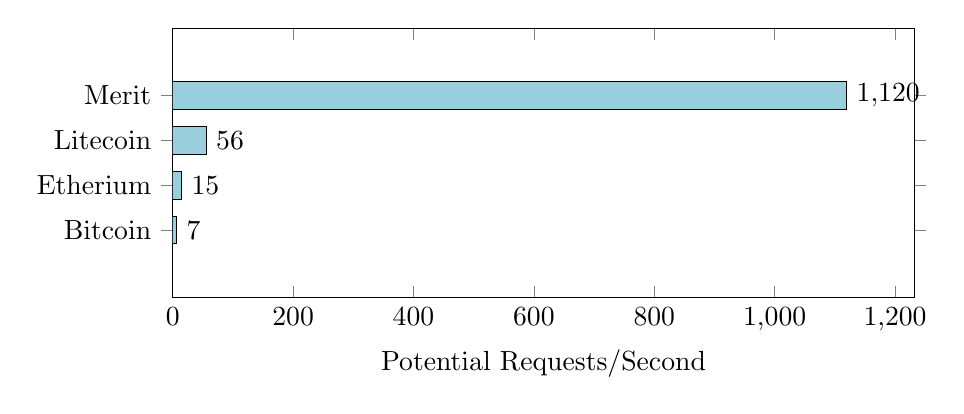
\begin{tikzpicture}
            \begin{axis}
                [xbar, xmin=0,
                width=11cm,
                height=5cm,
                enlarge y limits=0.5,
                xlabel={Potential Requests/Second},
                symbolic y coords={Bitcoin,Etherium,Litecoin,Merit},
                ytick=data,
                nodes near coords,
                nodes near coords align={horizontal}]
                \addplot [fill=merit] coordinates {(7,Bitcoin) (15,Etherium) (56,Litecoin) (1120,Merit)};
            \end{axis}
        \end{tikzpicture}
    \end{center}
    \caption{Stage One Transaction Rate}
\end{figure}

\subsubsection{Bandwidth}

In practice, the maximum block size might not be reached because of bandwidth limitations
in the network.  Research done in the Bitcoin Unlimited paper \cite{bitcoinunlimited} looks
at the impact of various block sizes.  Miners are at risk of creating orphaned blocks 
when as the size of blocks increases block because it takes some time for a block to propagate
across the network.  The larger the block size, the higher the chance the block will
compete with other blocks mined during the time it takes to propagate.

Therefore increasing block size beyond the network's capabilities to propagate blocks
provides no improvements over the transaction rate.  At some point, miners won't put more
transactions because the risk of creating stagnant blocks becomes too large.  A 
different method of increasing performance must, therefore, be considered.

\subsubsection{Lightning Network}

The Bitcoin lightning network attempts to offload transactions from the blockchain
to a network of channels.  The idea is that channels only need to announce final
results of all transactions on the blockchain once they are closed.  Any two parties
can send transactions to each other by routing the transactions through a series of
channels.  Unfortunately, there are several issues with the lighting network which
provide real-world limitations.

\begin{itemize}
    \item Opening and closing a channel requires staking coins in a funding transaction.
    \item Routing a transaction requires intermediaries to have the liquidity necessary
        to route transactions.
    \item The system is susceptible to DDOS attacks.
    \item The system is susceptible to fraud and may require users to use watchtower 
        nodes.
    \item The complexity of creating and maintaining a channel may mean it is appropriate for large institutions.
\end{itemize}

Merit is still evaluating whether it will incorporate lightning network features
into its system.

\subsection{Block Fabrics: A Generalization of the Nakamoto Blockchain}

A more dramatic approach needs to be taken to scale Merit for stage two because
increasing block size and frequency won't scale to support a sizeable worldwide user base.
The larger blocks and shorter block time will improve transaction rates over Bitcoin
and Ethereum, but is a fundamentally limited approach because the speed of the network
is only as fast as the speed of one machine on the network.  To achieve real scalability,
we need to design a system that has multiple writers by \gls{sharding} the address space
and converting a one-dimensional database into a two dimensional one.

The crucial insight is that the Nakamoto Blockchain is a degenerative case of what
we call \glspl{block fabric}, which are inspired by thousands of years of tradition from the
craft of weaving which create a form and structure of time.

\subsubsection{The Weave and Warp}

Merit implements an algorithm inspired by the weaving of fabrics.  Block fabrics
have many threads aligned in one direction in parallel called the \emph{Warp}
and these threads have a single thread woven through it back and forth called
the Weft.  In other words, many parallel strands are held together
by a single thread weaved through them over time.  Instead of calling this single 
thread the Weft, we will use the term the Weave to highlight the relationship
with time better.

\begin{figure}[H]
    \begin{center}
        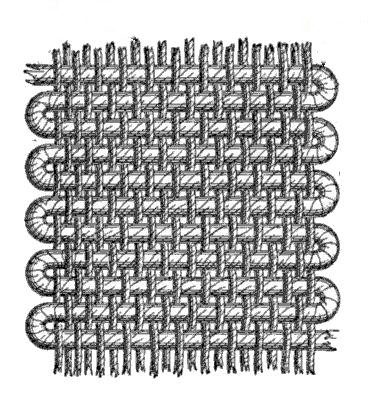
\includegraphics[scale=0.618]{fabric}
    \end{center}
    \caption{Weaving Fabric \cite{weave}}
\end{figure}

\subsubsection{Warp Chains}

Merit's sharding algorithm divides the address space into shards
called \emph{Warps}.  Each \emph{Warp} is a blockchain and has a single writer
for a period of time called the leader.  If we think of the Warp's existence in 
the platonic world, the Warp has existed from the beginning of time and will 
exist to the end of time.  In some sense, the Warp is independent of time similar
to how a real Warp on a loom is fixed before the weaving process begins, Yet the
fabric is wholly defined by time when it is woven.

Each miner competes to become the leader of a Warp by mining blocks on the \emph{Weave}.  An explanation of how the \emph{Weave} functions is described later.  Each \emph{Warp} has the following properties.

\begin{center}
    \scalebox{1.0}{
        \begin{tabular}{l|p{9cm}}
            Property & Description \\ \hline
            Blockchain & Each Warp is a blockchain.  \\
            Single Writer & A Warp has a single leader at any given time.  \\ 
            Prefix Range & Identity of a Warp is its address range.\\
            Many Warps & Number of Warps at any given time is defined.\\ 
            Have Transactions & Blocks in a Warp have transactions, invites, and beacons.  \\ 
            No PoW & Blocks do not have a proof-of-work.  \\ 
            Signed & Blocks are signed by the leader.\\ 
        \end{tabular}
    }
\end{center}

Each \gls{warp block} Has the following properties defined in the block header.

\begin{center}
    \scalebox{1.0}{
        \begin{tabular}{l|p{9cm}}
            Property & Description \\ \hline
            Previous Block & Hash to previous block in the warp.  \\
            Weave Block & Hash to weave block.  \\
            Merkel Root& Merkel Root hash describing the set of transactions\\ 
            Signature & The signature of the leader of the warp chain.\\
            Public Key & The public key of the leader of the warp chain.\\
        \end{tabular}
    }
\end{center}

Notice there is no nonce or proof of work in this chain.  The leader signs each block
and is allowed create as many blocks as possible that pass the address range validation
defined in the referenced \gls{weave block}.

\subsubsection{Prefix Range}

A Warp has a continuous address range with $N$ bytes in size.

\begin{center}
    \scalebox{1.0}{
        \begin{tabular}{l|p{9cm}}
            Property & Description \\ \hline
            Prefix Size & Number of bytes to match.  \\
            Start & Start of byte range.  \\
            End & End of byte range.  \\
        \end{tabular}
    }
\end{center}

The bytes that match against the address range are any bytes that are a permutation
between the start and end of the range.  Each Warp has a mutually exclusive 
address range assigned to it via the \emph{Weave} process described later.

\subsubsection{Warp Assignment Overview}

Each \emph{Warp} is a blockchain where each block contains transactions, invites,
and beacons that are assigned to it.  The \emph{Prefix Range} of the Warp is used in
the assignment algorithms to match the asset to the Warp.
The assignment logic for beacons, invites, and transactions is outlined in the table.

\begin{center}
    \scalebox{1.0}{
        \begin{tabular}{l|p{9cm}}
            Type & Assignment Logic\\ \hline
            Beacon & If the Beacon's address matches the Warp prefix \\
            Transaction & If one of the input's addresses matches the Warp prefix \\
            Invite & If one of the input's addresses matches the Warp prefix \\
        \end{tabular}
    }
\end{center}

\subsubsection{Invite and Transaction Assignment}

Invites and Transactions have the same structure, and therefore their assignment
to a Warp follows the same logic.  Merit inherits the transaction structure
of Bitcoin.  Each Transaction has one or more inputs and one or more outputs.
Each input references a previous output by transaction id and index.

\begin{figure}[H]
    \begin{center}
        \digraph[scale=0.618]{TA}{
            rankdir=TD;
            node [shape=record,style=filled,fillcolor="0.533333 0.314 0.87"];
            b [label="Transaction|Input Mgoc7q4w148kbajifJHryFwJiZgwm1z1gF"];
            w [label="Warp|{Start MgoXXXXXXXXXXXXXXXXXXXXXXXXXXXXXXX|End MgpXXXXXXXXXXXXXXXXXXXXXXXXXXXXXXX}"];
            b -> w [label="Assigned to"];
        }
    \end{center}
    \caption{Beacon Assignment}
\end{figure}

Each transaction input must have an address associated with it given the rules
of the Merit invite system.  A transaction is assigned to a Warp if it's input's
address matches a Warp's prefix.  Because most transactions have multiple inputs,
the transaction is split into many transactions. 

\subsubsection{Beacon Assignment}

It is vital that the Beacon ends up in the same Warp as the Invite that is
used to activate the Beacon.  Each Beacon has an address which it is advertising, and 
it is this address that an invite is sent.  The Beacon is matched to a Warp
by matching the Beacon's address to the Warp's address range.  Since Warps are 
guaranteed to have mutually exclusive prefixes, then the Beacon will end up 
in the same Warp as the Invite sent to it.

\begin{figure}[H]
    \begin{center}
        \digraph[scale=0.618]{BA}{
            rankdir=TD;
            node [shape=record,style=filled,fillcolor="0.533333 0.314 0.87"];
            b [label="Beacon| Address MEagc8eva9moLxkRi67GSL7AtVPdbyCYe5"];
            w [label="Warp|{Start MEagXXXXXXXXXXXXXXXXXXXXXXXXXXXXXX| End MEb1XXXXXXXXXXXXXXXXXXXXXXXXXXXXXX}"];
            b -> w [label="Assigned to"];
        }
    \end{center}
    \caption{Beacon Assignment}
\end{figure}

\subsubsection{Transaction Splitting}

Transactions with more than one input are split into many transactions with the same
outputs.  If a transaction has \emph{N} inputs, it will be split into \emph{N} transactions.  The original transaction fee is split among the Warps and rewarded to the Warp
leaders given the Warp fee rules.  The original transaction is considered complete when
all splits appear in blocks on their assigned Warps.

\begin{figure}[H]
    \begin{center}
        \digraph[scale=0.618]{TS}{
            rankdir=TD;
            node [shape=box,style=filled,fillcolor="0.533333 0.314 0.87"];
            t [label="Transaction with 3 inputs"];
            tc0 [label="Transaction with input 1"];
            tc1 [label="Transaction with input 2"];
            tc2 [label="Transaction with input 3"];
            w0 [label="Warp 1"];
            w1 [label="Warp 2"];
            w2 [label="Warp 3"];
            t -> tc0 [label="split"];
            t -> tc1 [label="split"];
            t -> tc2 [label="split"];
            tc0 -> w0 [label="assign"];
            tc1 -> w1 [label="assign"];
            tc2 -> w2 [label="assign"];
        }
    \end{center}
    \caption{Transaction Assignment}
\end{figure}

\subsubsection{The Weave Chain}

Miners compete on the Weave chain using the Cuckoo Cycle proof-of-work. 
The Weave can be thought of as the main blockchain.  It weaves through each Warp
in a deterministic order by partitioning the whole address space into \emph{N} warps.
The size of \emph{N} must be necessarily a power of two.  This means there can be,
2,4,8,...  Warps.  Each block in the Weave chain has three parts...

\begin{enumerate}
    \item Warp Owner Announcement.
    \item Merit Coinbase Transactions and Ambassador Rewards.
    \item Invite lottery rewards.
\end{enumerate}

The \gls{weave block} has the following data in the header.

\begin{center}
    \scalebox{1.0}{
        \begin{tabular}{l|p{9cm}}
            Property & Description \\ \hline
            Previous Block Hash & Hash to previous block in the warp.  \\
            Merkel Root Hash & Merkel Root hash describing the set of transactions.\\ 
            NBits & The number of leading zero bits the proof-of-work must have.  \\
            EdgeBits & The number of bits used to describe an edge cycle.  \\
            Nonce & An integer that is incremented to change the block hash.  \\
            Cycle & The proof-of-work in the form a Cuckoo Cycle.  \\
            Warp Number & Warp number.\\
            Total Warps & The total number of warps.\\
            Signature & The signature of the leader of the warp specified.\\
            Public Key & The public key of the leader of the warp specified.\\
        \end{tabular}
    }
\end{center}

The weave blocks require a \gls{proof-of-work} and are signed by the winning
writer of the \gls{warp} block.  Which warp they can write to is specified by the warp number
that is deterministically selected in a round robin fashion.

\begin{figure}[H]
    \begin{center}
        \digraph[scale=0.6]{WeaveBlocks}{
            graph [outputorder=nodesfirst overlap=false];
            rankdir=LR;
            node [shape=rectangle,style=filled,fillcolor="0.533333 0.314 0.87"];
            compound=true;
            splines=false;
            newrank=true;
            subgraph W {
                rank=source;
                e0 [label="Weave Block 1"];
                e1 [label="Weave Block 2"];
                e2 [label="Weave Block 3"];
                e3 [label="Weave Block 4"];
                e4 [label="Weave Block 5"];
                e5 [style=invis];
            }
            subgraph clusterA {
                label="Warp A";
                wA0 [label = "Block 1"];
                wA1 [label = "Block 2"];
                wA2 [label = "Block 3"];
            }
            subgraph clusterB {
                label="Warp B";
                wB0 [label = "Block 1"];
                wB1 [label = "Block 2"];
                wB2 [label = "Block 2"];
            }
            subgraph clusterC {
                label="Warp A";
                wA3 [label = "Block 1"];
                wA4 [label = "Block 2"];
                wA5 [label = "Block N"];
            }
            subgraph clusterD {
                label="Warp B";
                wB3 [label = "Block 4"];
                wB4 [label = "Block 5"];
                wB5 [label = "Block 6"];
            }
            subgraph clusterE {
                label="Warp A";
                wA6 [label = "Block 4"];
                wA7 [label = "Block 5"];
                wAN [label = "Block N"];
            }
            subgraph F {
                wB6 [style=invis label = "..."];
                wB7 [style=invis label = "..."];
                wBN [style=invis label = "..."];
            }

            {rank=sink;wA2;wB2;wA5;wB5;wAN;wBN;}

            e0 -> e1;
            e1 -> e2;
            e2 -> e3;
            e3 -> e4;
            e4 -> e5;
            e0 -> wA0 [weight=100 lhead=clusterA];
            wA0 -> wA1;
            wA1 -> wA2;
            wA2 -> wA3 [constraint=false];
            e1 -> wB0 [weight=100 lhead=clusterB];
            wB0 -> wB1;
            wB1 -> wB2;
            wB2 -> wB3 [constraint=false];
            e2 -> wA3 [weight=100 lhead=clusterC];
            wA3 -> wA4;
            wA4 -> wA5;
            wA5 -> wA6 [constraint=false];
            e3 -> wB3 [weight=100 lhead=clusterD];
            wB3 -> wB4;
            wB4 -> wB5;
            wB5 -> wB6 [constraint=false];
            e4 -> wA6 [weight=100 lhead=clusterE];
            wA6 -> wA7;
            wA7 -> wAN;
            e5 -> wB6 [weight=100 style=invis lhead=clusterF];
            wB6 -> wB7[style=invis];
            wB7 -> wBN[style=invis];
        }
    \end{center}
    \caption{Weave and Warp}
\end{figure}


\subsubsection{Warp Owner Announcement}

When miners successfully mine a block on the Weave chain, they take over being
the write to a Warp that is deterministically determined by taking the next Warp
in the set of $N$ Warps that are assigned at the time.  If we assign each
Warp an index $W$ into the set of $N$, and any given block $B_{i}$ returns the assigned warp index $W$ with the function $A(i)$.  The Warp assigned to block $B_{i}$ is 

    $$A(i) = A(i-1)+1 \mod N$$.

\subsubsection{Address Space Partitioning}

Just like Bitcoin, Merit addresses are a RIPEMD-160 hash function which is a 160-bit
hash.  This is a huge space and is broken up into any practical number
of pieces of equal shards.  The size of each shard can be easily specified by the
number of significant bits required to describe the start and end of each shard.
Since we don't expect the number of shards to be too significant at any given time,
then the address range can be compactly stored using the minimum number of bits
required to define the start and end of the range.

\begin{figure}[H]
    \begin{center}
        \digraph[scale=0.618]{FourAddressSpace}{
            rankdir=TD;
            node [shape=record,style=filled,fillcolor="0.533333 0.314 0.87"];
            subgraph cluster4 {
                rank=source;
                w0 [label="{Warp 1|{00|01}}"];
                w1 [label="{Warp 2|{01|10}}"];
                w2 [label="{Warp 3|{10|11}}"];
                w3 [label="{Warp 3|{11|00}}"];
            }
            space -> w0;
            space -> w1;
            space -> w2;
            space -> w3;
            subgraph {
                rank=sink;
                space [label="160-bit Address Space"];
            }
        }
    \end{center}
    \caption{Four Warp Partitioning}
\end{figure}

\subsubsection{Dynamic Warp Adjustment}

The number of Warps can be adjusted dynamically by looking at the transaction
rate over the last \emph{X} blocks.  We can decide what \emph{At Capacity} is per
Warp, and use that to maintain enough Warps never to surpass this capacity.  These
attributes can be fixed to create a deterministic algorithm for determining the
number of Warps at any given block on the Weave chain.  When the number of Warps 
\emph{N} increases from one block to the next, the new Warp assignment will assign
only part of the previous Warp.  In this situation, the new Warp partially occludes
a previous Warp.  Each warp leader must watch the Weave blockchain to understand 
when their Warp is partially occluded.  Any Warp blocks after the block referenced
in the occluding Weave block must not have transactions that are occluded.  This
may require the occluded warp leader to abandon any blocks after the referenced
block and start writing again.

\subsubsection{Coinbase Transactions and Ambassador Rewards}

Coinbase transactions, Ambassador Rewards, and invite generation occur on the
Weave chain.  This makes sense because these transactions have no inputs and
therefore cannot be assigned to a Warp.  This rule also requires changes in the
existing blockchain algorithm defined in stage one scaling where Merit is a single
blockchain with 16MB blocks and one minute block time.

\subsubsection{Warp Fee Payout}

To incentivize future leaders of a Warp to pick the latest block written
by the previous Warp leader, the previous leader will give 60\% of the fees they
accumulated to the next leader and keep 40\%.  This 40/60 split is inspired by
the Bitcoin-NG \cite{bitcoinng} paper.  The Bitcoin-NG paper assumes an attacker
is bounded by 1/4th of the mining power.  However, because Warps partition the
address space, and therefore the fee distribution, the attacker has a smaller
incentive to misbehave because the fees from all transactions are distributed
among all leaders.  The attacker must have a sustained attack over the period of
$N*2$ Weave blocks where $N$ is the number of Warps to capture 100\% of the
transaction fees for an $N$ block period.

\subsubsection{Fabric Analysis}

Looking back at the two concepts, we can summarize by saying that the Weave
assigns leadership of writing capability to a Warp to the miner who wins a Weave block.
They can write to the Warp until another leader of the Warp takes over.  The assignment
of the Warps is well defined and ordered where the time between Warp leadership
changing hands is regular.  For example, if the number of Warps available is $N$, then
a Warp leader will expect to lose leadership of the Warp in $N$ minutes.  This
is because the time between blocks on the Weave chain is one minute. 

\begin{figure}[H]
        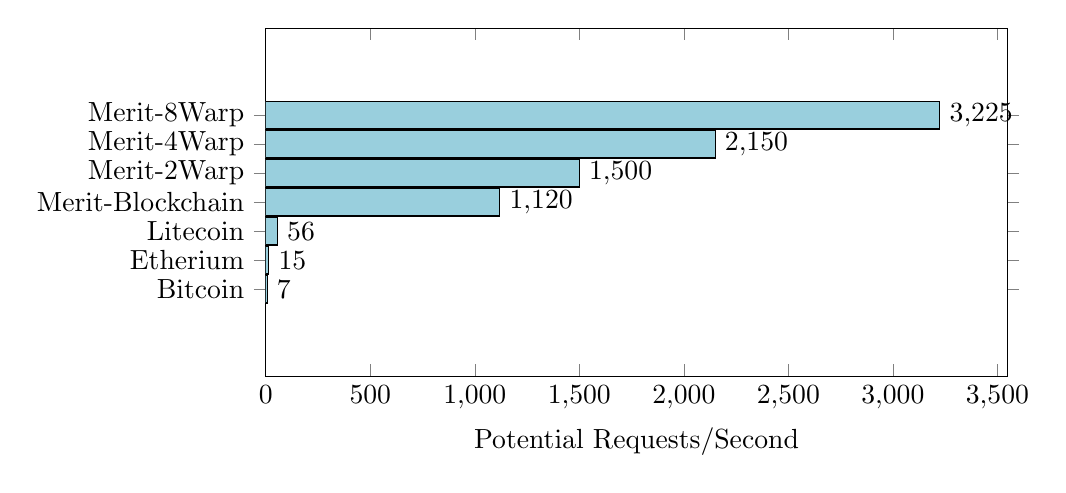
\begin{tikzpicture}
            \begin{axis}
                [xbar, xmin=0,
                width=11cm,
                height=6cm,
                enlarge y limits=0.5,
                xlabel={Potential Requests/Second},
                symbolic y coords={Bitcoin,Etherium,Litecoin,Merit-Blockchain,Merit-2Warp,Merit-4Warp,Merit-8Warp},
                ytick=data,
                nodes near coords,
                nodes near coords align={horizontal}]
                \addplot [fill=merit] coordinates {(7,Bitcoin) (15,Etherium) (56,Litecoin) (1120,Merit-Blockchain) (1500,Merit-2Warp) (2150,Merit-4Warp) (3225,Merit-8Warp)};
            \end{axis}
        \end{tikzpicture}
    \caption{Stage Two Transaction Rate}
\end{figure}

There is a constant balance between increasing throughput or reducing latency.
Merit attempts to reduce latency by providing fast minute block times on the Weave
blockchain.  At the same time, throughput is increased by having multiple writers
committing transactions on the blockchain.  A downside is that transaction on a given
Warp are confirmed for every $N$ blocks where $N$ is the count of Warps.  This is
because transactions from a particular reader are committed to the blockchain once
the next leader for that Warp acknowledges the blocks of the current leader by
mining a block no the Weave chain.  This means that latency of confirming transactions
is highly predictable and is a function of the number of Warps $N$ and the time
between blocks on the Weave.  As an illustrative example, if $N$ is two, then the
latency when a Warps transactions are committed is two minutes.  As the system reaches
capacity, $N$ would be doubled to four and therefore the confirmation time would
increase to four minutes.  When $N$ reaches 64, we end up with a confirmation time
around an hour.  The relation between throughput is geometrically defined via the
space-time relation of the Weave and Warp chains.

As an illustrate example, if we say each Warp leader is capable of writing 1K split
transactions per second, and likely 100\% of those transactions created from a
transaction with at least two inputs, then we can say the overall transaction
throughput is 1/2 of the Warp transaction throughput.  So with 2 Warps, we have
an overall rate of 1000 transactions per second because $1000 = 2000/2$.  Four
Warps would double the transaction rate to 2K transactions per second.  It is 
easy to see how only having a few Warps can increase the transaction rate
significantly.  However, it is important to note here that this assumes transactions
with only two inputs.  With more substantial transactions, the throughput will not
double so cleanly.  The dynamic warp adjustment algorithm should compensate for
this and provision enough warps to handle the required transaction volume.  An
analysis of the average input size once Merit has grown would provide a chance
for a better analysis.

The obvious take away here is that eventually for any machine to have a set of
all the unspent outputs (UTXOs), it would eventually need to index all the
transactions in the system.However, this process can be much faster than the
original block generation process of the Warp leaders.  This is because the Warp
leaders do more work because they have to decide which transactions to put in a Warp.

\section{Summary}

Merit has aggressively focused on community, ease of use, safety, and scalability in an
attempt to tackle the centralization and trust in third-parties that have corrupted
the vision of the cryptographic currency community.

Merit recognizes that there is a wide variety of users of the system and introduces
incentives to those ambassadors of the system that go beyond mining.  By having
an Ambassador Tree, we allow users to support people and organizations they love
without having to understand and manage complex software systems.

\clearpage
\printglossaries

\begin{thebibliography}{1}


\bibitem{drypool}
    Aron Laszka, Benjamin Johnson, and Jens Grossklags,
    \textit{When Bitcoin Mining Pools Run Dry},
    Financial Cryptography and Data Security: FC 2015 International Workshops, 
    January 30, 2015, Revised Selected Papers (pp.63-77)

\bibitem{cuckoo}
    Tromp,
    \textit{Cuckoo Cycle},
    https://github.com/tromp/cuckoo/

\bibitem{poisson}
    F.  C.  Kingman,
    \textit{Poisson Processes},
    (17 December 1992) Clarendon Press,
    ISBN 978-0-19-159124-2

\bibitem{bitpoisson}
    Pranav Gokhale,
    \textit{Why is the Poisson distribution relevant to Bitcoin/blockchain?},
    https://www.quora.com/Why-is-the-Poisson-distribution-relevant-to-Bitcoin-blockchain,
    Feb 21, 2017

\bibitem{ripemd}
    Antoon Bosselaers, and Bart Preneel,
    \textit{The hash function RIPEMD-160},
    https://homes.esat.kuleuven.be/~bosselae/ripemd160.html

\bibitem{IDNA}
    P.  Faltstrom, Ed., 
    \textit{The Unicode Code Points and Internationalized Domain Names for 
        Applications (IDNA)},
    https://tools.ietf.org/html/rfc5892,
    August 2010 ISSN: 2070-1721

\bibitem{stringprep}
    Blanchet Viagenie,
    \textit{Preparation of Internationalized Strings ("stringprep")},
    https://tools.ietf.org/html/rfc3454,
    December 2002

\bibitem{homograph}
    Evgeniy Gabrilovich Alex Gontmakher,
    \textit{The Homograph Attack},
    http://www.cs.technion.ac.il/~gabr/papers/homograph\_full.pdf,
    Communications of the ACM, 45(2):128, February 2002

\bibitem{phishing}
    Mark Maunder,
    \textit{Chrome and Firefox Phishing Attack Uses Domains Identical to Known Safe Sites},
    https://www.wordfence.com/blog/2017/04/chrome-firefox-unicode-phishing/,
    April 14, 2017

\bibitem{siphash}
    Jean-Philippe Aumasson and Daniel J.  Bernstein,
    \textit{SipHash: a fast short-input PRF},
    https://131002.net/siphash/siphash.pdf

\bibitem{inverse}
    Luc Devroye,
    \textit{Non-Uniform Random Variate Generation},
    http://www.eirene.de/Devroye.pdf,
    New York: Springer-Verlag.  1986

\bibitem{scripts}
    \textit{Script},
    https://en.bitcoin.it/wiki/Script

\bibitem{ddos}
    E.  Rescorla, Ed.,
    \textit{Internet Denial-of-Service Considerations},
    https://tools.ietf.org/html/rfc4732,
    November 2006

\bibitem{eframspirakis}
    Efraimidis and Spirakis,
    \textit{Weighted random sampling with a reservoir},
    https://doi.org/10.1016/j.ipl.2005.11.003,
    Information Processing Letters,
    Volume 97, Issue 5, 16 March 2006, Pages 181-185

\bibitem{avalanceh}
    Horst Feistel,
    \textit{Cryptography and Computer Privacy},
    http://www.apprendre-en-ligne.net/crypto/bibliotheque/feistel/index.html,
    Scientific American, May 1973, Volume 228, No 5, pp.  15-23

\bibitem{fees}
    Alyssa Hertig,
    \textit{Bitcoin Fees Are Down Big: Why It Happened And What It Means},
    https://www.coindesk.com/bitcoin-low-fees-why-happening-why-matters/,
    Feb 23, 2018, at 01:30 UTC

\bibitem{bitcoinunlimited}
    Peter R.  Rizun,
    \textit{A Transaction Fee Market Exists Without a Block Size Limit},
    https://www.bitcoinunlimited.info/resources/feemarket.pdf

\bibitem{ethereumscale}
    Coindesk
    \textit{How Will Ethereum Scale?},
    https://www.coindesk.com/information/will-ethereum-scale/

\bibitem{weave}
    Wikipedia,
    \textit{Warp and weft.jpg},
    https://en.wikipedia.org/wiki/File:Warp\_and\_weft.jpg

\bibitem{bitcoinng}
    Ittay Eyal, Adem Efe Gence r, Emin Gün Sire r, and Robbert van Renesse, Cornell University,
    \textit{Bitcoin-NG: A Scalable Blockchain Protocol},
    https://www.usenix.org/system/files/conference/nsdi16/nsdi16-paper-eyal.pdf

\bibitem{uri}
    T.  Berners-Lee, R.  Fielding, L.  Masinter,
    \textit{Uniform Resource Identifiers (URI): Generic Syntax},
    http://www.rfc-base.org/txt/rfc-2396.txt

\bibitem{avalanche}
    By Horst Feistel,
    \textit{Cryptography and Computer Privacy},
    http://www.apprendre-en-ligne.net/crypto/bibliotheque/feistel/index.html

\bibitem{PageRank}
    Sergey Brin, Lawrence Page,
    \textit{The Anatomy of a Large-Scale Hypertextual
Web Search Engine},
    http://ilpubs.stanford.edu:8090/361/1/1998-8.pdf

\bibitem{pachira}
     John (JD) Douceur, Thomas Moscibroda ,
    \textit{Lottery Trees: Motivational Deployment of Networked Systems},
    SIGCOMM 2007: ACM SIGCOMM Conference on Applications, Technologies,
    Architectures, and Protocols for Computer Communications, Kyoto, Japan 

\end{thebibliography}
\end{document}
